\documentclass[OPS,toc,SOW]{lsstdoc}
\input{meta.tex}

\usepackage{pdflscape}
\usepackage{afterpage}
\usepackage{arydshln}
\usepackage[colorinlistoftodos]{todonotes}
\usepackage[
singlelinecheck=false % <-- important
]{caption}

% DO NOT EDIT - generated by /Users/womullan/LSSTgit/lsst-texmf/bin/generateAcronyms.py from https://lsst-texmf.lsst.io/.
\newacronym{AD} {AD} {Associate \gls{Director}}
\newacronym{AP} {AP} {\gls{Alert Production}}
\newacronym{APDB} {APDB} {\gls{Alert Production DataBase}}
\newacronym{API} {API} {Application Programming Interface}
\newacronym{AURA} {AURA} {\gls{Association of Universities for Research in Astronomy}}
\newglossaryentry{Alert} {name={Alert}, description={A packet of information for each source detected with signal-to-noise ratio > 5 in a difference image by Alert Production, containing measurement and characterization parameters based on the past 12 months of LSST observations plus small cutouts of the single-visit, template, and difference images, distributed via the internet}}
\newglossaryentry{Alert Production} {name={Alert Production}, description={Executing on the Prompt Processing system, the Alert Production payload processes and calibrates incoming images, performs Difference Image Analysis to identify DIASources and DIAObjects, and then packages the resulting alerts for distribution.}}
\newglossaryentry{Alert Production DataBase} {name={Alert Production DataBase}, description={A dedicated, internal database system used to support LSST Alert Production.  Does not support end-user access.}}
\newglossaryentry{Alternate Standard Visit} {name={Alternate Standard Visit}, description={A single observation of an LSST field comprised of one 30 second exposure}}
\newglossaryentry{Archive} {name={Archive}, description={The repository for documents required by the NSF to be kept. These include documents related to design and development, construction, integration, test, and operations of the LSST observatory system. The archive is maintained using the enterprise content management system DocuShare, which is accessible through a link on the project website www.project.lsst.org}}
\newglossaryentry{Archive Center} {name={Archive Center}, description={Part of the LSST Data Management System, the LSST archive center is a data center at NCSA that hosts the LSST Archive, which includes released science data and metadata, observatory and engineering data, and supporting software such as the LSST Software Stack}}
\newglossaryentry{Association Pipeline} {name={Association Pipeline}, description={An application that matches detected Sources or DIASources or generated Objects to an existing catalog of Objects, producing a (possibly many-to-many) set of associations and a list of unassociated inputs. Association Pipelines are used in Alert Production after DIASource generation and in the final stages of Data Release processing to ensure continuity of Object identifiers}}
\newglossaryentry{Association of Universities for Research in Astronomy} {name={Association of Universities for Research in Astronomy}, description={ consortium of US institutions and international affiliates that operates world-class astronomical observatories, AURA is the legal entity responsible for managing what it calls independent operating Centers, including LSST, under respective cooperative agreements with the National Science Foundation. AURA assumes fiducial responsibility for the funds provided through those cooperative agreements. AURA also is the legal owner of the AURA Observatory properties in Chile}}
\newglossaryentry{Authentication} {name={Authentication}, description={The action of demonstrating who you are and an person, mission, or other entity. Usually by use of a password or security token}}
\newacronym{B} {B} {Byte (8 bit)}
\newacronym{BCE} {BCE} {Before Common Era}
\newglossaryentry{Base Facility} {name={Base Facility}, description={The data center located at the Base Site in La Serena, Chile. The Base Facility is composed of the Base portion of the Prompt Enclave directly supporting Observatory operations, the Commissioning Cluster, an Archive Enclave holding data products, and the Chilean Data Access Center}}
\newglossaryentry{Batch Production} {name={Batch Production}, description={Computational processing that is executed as inputs become available, in a distributed way across multiple enclaves when needed, while tracking status and outputs. Examples of Batch Production include offline processing for Prompt Data Products, calibration products, template images, and Special Programs data products. Prioritization protocols for the various types of batch production are given in LDM-148}}
\newglossaryentry{Butler} {name={Butler}, description={A middleware component for persisting and retrieving image datasets (raw or processed), calibration reference data, and catalogs}}
\newacronym{CA} {CA} {Control (or Cost) Account}
\newacronym{CCB} {CCB} {\gls{Change Control Board}}
\newacronym{CCD} {CCD} {\gls{Charge-Coupled Device}}
\newacronym{CERN} {CERN} {European Organization for Nuclear Research}
\newacronym{CI} {CI} {Continuous Integration}
\newacronym{CPU} {CPU} {Central Processing Unit}
\newglossaryentry{Calibration Image} {name={Calibration Image}, description={Any of a set of images used in the Instrument Signature Removal pipeline to remove distortions caused by the telescope, detector, or other sources, from the raw images. Includes darks, flats, tunable-laser dome flats, etc}}
\newglossaryentry{Camera} {name={Camera}, description={The LSST subsystem responsible for the 3.2-gigapixel LSST camera, which will take more than 800 panoramic images of the sky every night. SLAC leads a consortium of Department of Energy laboratories to design and build the camera sensors, optics, electronics, cryostat, filters and filter exchange mechanism, and camera control system}}
\newglossaryentry{Center} {name={Center}, description={An entity managed by AURA that is responsible for execution of a federally funded project}}
\newglossaryentry{Change Control Board} {name={Change Control Board}, description={Advisory board to the Project Manager; composed of technical and management representatives who recommend approval or disapproval of proposed changes to, deviations from, and waivers to a configuration item's current approved configuration documentation}}
\newglossaryentry{Charge-Coupled Device} {name={Charge-Coupled Device}, description={a particular kind of solid-state sensor for detecting optical-band photons. It is composed of a 2-D array of pixels, and one or more read-out amplifiers}}
\newglossaryentry{Citizen Science} {name={Citizen Science}, description={the collection and analysis of data relating to the natural world by members of the general public, typically as part of a collaborative project with professional scientists.}}
\newacronym{ComCam} {ComCam} {The commissioning \gls{camera} is a single-raft, 9-CCD \gls{camera} that will be installed in LSST during commissioning, before the final \gls{camera} is ready.}
\newglossaryentry{Commissioning} {name={Commissioning}, description={A two-year phase at the end of the Construction project during which a technical team a) integrates the various technical components of the three subsystems; b) shows their compliance with ICDs and system-level requirements as detailed in the LSST Observatory System Specifications document (OSS, LSE-30); and c) performs science verification to show compliance with the survey performance specifications as detailed in the LSST Science Requirements Document (SRD, LPM-17)}}
\newglossaryentry{Construction} {name={Construction}, description={The period during which LSST observatory facilities, components, hardware, and software are built, tested, integrated, and commissioned. Construction follows design and development and precedes operations. The LSST construction phase is funded through the NSF MREFC account}}
\newacronym{DAC} {DAC} {\gls{Data Access Center}}
\newacronym{DB} {DB} {DataBase}
\newacronym{DBB} {DBB} {\gls{Data Backbone}}
\newacronym{DC2} {DC2} {Data Challenge 2 (\gls{DESC})}
\newacronym{DCR} {DCR} {\gls{Differential Chromatic Refraction}}
\newacronym{DECam} {DECam} {Dark Energy \gls{Camera}}
\newacronym{DESC} {DESC} {Dark Energy \gls{Science Collaboration}}
\newacronym{DF} {DF} {Data Facility}
\newacronym{DIA} {DIA} {\gls{Difference Image Analysis}}
\newglossaryentry{DIAObject} {name={DIAObject}, description={A DIAObject is the association of DIASources, by coordinate, that have been detected with signal-to-noise ratio greater than 5 in at least one difference image. It is distinguished from a regular Object in that its brightness varies in time, and from a SSObject in that it is stationary (non-moving)}}
\newglossaryentry{DIASource} {name={DIASource}, description={A DIASource is a detection with signal-to-noise ratio greater than 5 in a difference image}}
\newacronym{DM} {DM} {\gls{Data Management}}
\newacronym{DMS} {DMS} {\gls{Data Management Subsystem}}
\newacronym{DMS-REQ} {DMS-REQ} {Data Management System Requirements prefix}
\newacronym{DMSR} {DMSR} {DM System Requirements; \gls{LSE}-61}
\newacronym{DMTN} {DMTN} {DM Technical Note}
\newacronym{DNS} {DNS} {Domain Name Service}
\newacronym{DOE} {DOE} {\gls{Department of Energy}}
\newacronym{DP} {DP} {Data Production}
\newacronym{DP0} {DP0} {Data Preview 0}
\newacronym{DP1} {DP1} {Data Preview 1}
\newacronym{DP2} {DP2} {Data Preview 2}
\newacronym{DPDD} {DPDD} {Data Product Definition \gls{Document}}
\newacronym{DR} {DR} {\gls{Data Release}}
\newacronym{DR1} {DR1} {Data \gls{Release} 1}
\newacronym{DRP} {DRP} {\gls{Data Release Production}}
\newglossaryentry{Data Access Center} {name={Data Access Center}, description={Part of the LSST Data Management System, the US and Chilean DACs will provide authorized access to the released LSST data products, software such as the Science Platform, and computational resources for data analysis. The US DAC also includes a service for distributing bulk data on daily and annual (Data Release) timescales to partner institutions, collaborations, and LSST Education and Public Outreach (EPO). }}
\newglossaryentry{Data Backbone} {name={Data Backbone}, description={The software that provides for data registration, retrieval, storage, transport, replication, and provenance capabilities that are compatible with the Data Butler. It allows data products to move between Facilities, Enclaves, and DACs by managing caches of files at each endpoint, including persistence to long-term archival storage (e.g. tape)}}
\newglossaryentry{Data Management} {name={Data Management}, description={The LSST Subsystem responsible for the Data Management System (DMS), which will capture, store, catalog, and serve the LSST dataset to the scientific community and public. The DM team is responsible for the DMS architecture, applications, middleware, infrastructure, algorithms, and Observatory Network Design. DM is a distributed team working at LSST and partner institutions, with the DM Subsystem Manager located at LSST headquarters in Tucson}}
\newglossaryentry{Data Management Subsystem} {name={Data Management Subsystem}, description={The Data Management Subsystem is one of the four subsystems which constitute the LSST Construction Project. The Data Management Subsystem is responsible for developing and delivering the LSST Data Management System to the LSST Operations Project}}
\newglossaryentry{Data Management System} {name={Data Management System}, description={The computing infrastructure, middleware, and applications that process, store, and enable information extraction from the LSST dataset; the DMS will process peta-scale data volume, convert raw images into a faithful representation of the universe, and archive the results in a useful form. The infrastructure layer consists of the computing, storage, networking hardware, and system software. The middleware layer handles distributed processing, data access, user interface, and system operations services. The applications layer includes the data pipelines and the science data archives' products and services}}
\newglossaryentry{Data Product} {name={Data Product}, description={The LSST survey will produce three categories of Data Products. Prompt, Data Release, User Generated. Previously referred to as Levels 1, 2, and 3}}
\newglossaryentry{Data Release} {name={Data Release}, description={The approximately annual reprocessing of all LSST data, and the installation of the resulting data products in the LSST Data Access Centers, which marks the start of the two-year proprietary period}}
\newglossaryentry{Data Release Data Product} {name={Data Release Data Product}, description={These products will be made available annually as the result of coherent processing of the entire science data set to date. These will include calibrated images; measurements of positions, fluxes, and shapes; variability information such as orbital parameters for moving objects; and an appropriate compact description of light curves. The Data Release Data Products will include a uniform reprocessing of the difference-imaging-based Prompt Data Products}}
\newglossaryentry{Data Release Processing} {name={Data Release Processing}, description={Deprecated term; see Data Release Production}}
\newglossaryentry{Data Release Production} {name={Data Release Production}, description={An episode of (re)processing all of the accumulated LSST images, during which all output DR data products are generated. These episodes are planned to occur annually during the LSST survey, and the processing will be executed at the Archive Center. This includes Difference Imaging Analysis, generating deep Coadd Images, Source detection and association, creating Object and Solar System Object catalogs, and related metadata}}
\newglossaryentry{Department of Energy} {name={Department of Energy}, description={cabinet department of the United States federal government; the DOE has assumed technical and financial responsibility for providing the LSST camera. The DOE's responsibilities are executed by a collaboration led by SLAC National Accelerator Laboratory}}
\newglossaryentry{Difference Image} {name={Difference Image}, description={Refers to the result formed from the pixel-by-pixel difference of two images of the sky, after warping to the same pixel grid, scaling to the same photometric response, matching to the same PSF shape, and applying a correction for Differential Chromatic Refraction. The pixels in a difference thus formed should be zero (apart from noise) except for sources that are new, or have changed in brightness or position. In the LSST context, the difference is generally taken between a visit image and template. }}
\newglossaryentry{Difference Image Analysis} {name={Difference Image Analysis}, description={The detection and characterization of sources in the Difference Image that are above a configurable threshold, done as part of Alert Generation Pipeline}}
\newglossaryentry{Differential Chromatic Refraction} {name={Differential Chromatic Refraction}, description={The refraction of incident light by Earth's atmosphere causes the apparent position of objects to be shifted, and the size of this shift depends on both the wavelength of the source and its airmass at the time of observation. DCR corrections are done as a part of DIA}}
\newglossaryentry{Director} {name={Director}, description={The person responsible for the overall conduct of the project; the LSST director is charged with ensuring that both the scientific goals and management constraints on the project are met. S/he is the principal public spokesperson for the project in all matters and represents the project to the scientific community, AURA, the member institutions of LSSTC, and the funding agencies}}
\newglossaryentry{Docker} {name={Docker}, description={A system for packaging and distributing software using self-contained containers which may be run on any Linux system; \url{https://www.docker.com/}}}
\newglossaryentry{DocuShare} {name={DocuShare}, description={The trade name for the enterprise management software used by LSST to archive and manage documents}}
\newglossaryentry{Document} {name={Document}, description={Any object (in any application supported by DocuShare or design archives such as PDMWorks or GIT) that supports project management or records milestones and deliverables of the LSST Project}}
\newacronym{EFD} {EFD} {Engineering and Facility Database}
\newacronym{EPO} {EPO} {\gls{Education and Public Outreach}}
\newacronym{ESNet} {ESNet} {Energy Sciences Network}
\newglossaryentry{Education and Public Outreach} {name={Education and Public Outreach}, description={The LSST subsystem responsible for the cyberinfrastructure, user interfaces, and outreach programs necessary to connect educators, planetaria, citizen scientists, amateur astronomers, and the general public to the transformative LSST dataset}}
\newglossaryentry{Enclave} {name={Enclave}, description={Individually defined portions of the computational resources at the Summit, Base, NCSA, and Satellite Facilities, such as the Prompt Enclave, the Archive Enclave, etc. }}
\newacronym{FITS} {FITS} {\gls{Flexible Image Transport System}}
\newacronym{FLOPS} {FLOPS} {FLoating point Operation per Second}
\newacronym{FOA} {FOA} {Funding \gls{Opportunity} Announcement}
\newacronym{FY23} {FY23} {Financial Year 23}
\newglossaryentry{Flexible Image Transport System} {name={Flexible Image Transport System}, description={an international standard in astronomy for storing images, tables, and metadata in disk files. See the IAU FITS Standard for details}}
\newglossaryentry{ForcedSource} {name={ForcedSource}, description={DRP table resulting from forced photometry}}
\newacronym{GB} {GB} {Gigabyte}
\newacronym{GID} {GID} {Group Identifier}
\newacronym{GNU} {GNU} {GNU's Not Unix! An operating system and an extensive collection of free computer \gls{software}}
\newacronym{GPL} {GPL} {GNU Public License}
\newacronym{Gb} {Gb} {Gigabit}
\newacronym{HSC} {HSC} {Hyper Suprime-Cam}
\newglossaryentry{Handle} {name={Handle}, description={The unique identifier assigned to a document uploaded to DocuShare}}
\newacronym{IAU} {IAU} {International Astronomical Union}
\newacronym{ICD} {ICD} {\gls{Interface Control Document}}
\newacronym{IN2P3} {IN2P3} {Institut National de Physique Nucléaire et de Physique des Particules}
\newacronym{IP} {IP} {Internet Protocol}
\newacronym{IT} {IT} {Information Technology}
\newacronym{ITC} {ITC} {Information Technology \gls{Center}}
\newacronym{IVOA} {IVOA} {International Virtual-Observatory Alliance}
\newglossaryentry{Instrument Signature Removal} {name={Instrument Signature Removal}, description={Instrument Signature Removal is a pipeline that applies calibration reference data in the course of raw data processing, to remove artifacts of the instrument or detector electronics, such as removal of overscan pixels, bias correction, and the application of a flat-field to correct for pixel-to-pixel variations in sensitivity}}
\newglossaryentry{Interface Control Document} {name={Interface Control Document}, description={A Document that describes, defines, and controls the interface(s) of a system, thereby bounding its requirements. The description includes the inputs and outputs of a single system or element. An ICD may also describe the interface between two systems or subsystems. The purpose of the ICD is to communicate all possible inputs to and all potential outputs from a system for some potential or actual user of the system in operations. The internal interfaces of a system or subsystem are typically not documented in an ICD, but rather in a system design document}}
\newglossaryentry{J2000} {name={J2000}, description={Julian Date referring to the instant of 12 noon (midday) on January 1, 2000. IAU standard equinox.}}
\newacronym{JD} {JD} {\gls{Julian Date}}
\newglossaryentry{JIRA} {name={JIRA}, description={issue tracking product (not an acronym but a truncation of Gojira the Japanese name for Godzilla)}}
\newglossaryentry{Julian Date} {name={Julian Date}, description={The Julian Date (JD) of any instant is the Julian day number for the preceding noon (UTC), plus the fraction of the day elapsed since that instant. The Julian day number is a running sequence of integral days, starting at noon, since the beginning of the Julian Period; JD 0.0 corresponds to noon on 1 January 4713 BCE. Various Julian Date converters are available on the Web. For example, 18h 00m 00.0s UT on 2014-July-01 (near the start of LSST construction) corresponds to JD 2456840.25}}
\newacronym{K8S} {K8S} {Kubernetes provisioning system}
\newacronym{KB} {KB} {KiloByte}
\newglossaryentry{Kubernetes} {name={Kubernetes}, description={A system for automating application deployment and management using software containers (e.g. Docker); \url{https://kubernetes.io}}}
\newacronym{LATISS} {LATISS} {LSST Atmospheric Transmission Imager and Slitless Spectrograph}
\newacronym{LCR} {LCR} {\gls{LSST Change Request}}
\newacronym{LDF} {LDF} {LSST Data Facility}
\newacronym{LDM} {LDM} {LSST Data Management (Document \gls{Handle})}
\newacronym{LDO} {LDO} {LSST Document \gls{Operations} (Document Handle)}
\newacronym{LHN} {LHN} {Long Haul Network}
\newacronym{LOY1} {LOY1} {LSST \gls{Operations} Year 1}
\newacronym{LPM} {LPM} {LSST Project Management (Document \gls{Handle})}
\newacronym{LSE} {LSE} {LSST \gls{Systems Engineering} (Document Handle)}
\newacronym{LSP} {LSP} {LSST \gls{Science Platform} (now Rubin \gls{Science Platform})}
\newacronym{LSST} {LSST} {Legacy Survey of Space and Time (formerly Large Synoptic Survey Telescope)}
\newglossaryentry{LSST Change Request} {name={LSST Change Request}, description={document that proposes a change to a configuration item; after evaluation by the CCB and decision by the Project Manager, the change request is updated with the outcome, action items, and necessary notification}}
\newglossaryentry{LSST Corporation} {name={LSST Corporation}, description={An Arizona 501(c)3 not-for-profit corporation formed in 2003 for the purpose of designing, constructing, and operating the LSST System. During design and development, the Corporation stewarded private funding used for such essential contributions as early site preparation, mirror construction, and early data management system development. During construction, LSSTC will secure private operations funding from international affiliates and play a key role in preparing the scientific community to use the LSST dataset}}
\newglossaryentry{LSST Project Office} {name={LSST Project Office}, description={Official name of the stand-alone AURA operating center responsible for execution of the LSST construction project under the NSF MREFC account}}
\newglossaryentry{LSST Science Pipelines} {name={LSST Science Pipelines}, description={software used to perform the LSST data reduction pipelines.lsst.io}}
\newacronym{LSSTC} {LSSTC} {\gls{LSST Corporation}}
\newacronym{LSSTPO} {LSSTPO} {\gls{LSST Project Office}}
\newglossaryentry{Level 1 Data Product} {name={Level 1 Data Product}, description={Deprecated term; see Prompt Data Product}}
\newglossaryentry{Level 3 Data Product} {name={Level 3 Data Product}, description={Deprecated term; see User Generated Data Product}}
\newacronym{MB} {MB} {MegaByte}
\newacronym{MPC} {MPC} {Minor Planet \gls{Center}}
\newacronym{MREFC} {MREFC} {\gls{Major Research Equipment and Facility Construction}}
\newglossaryentry{Major Research Equipment and Facility Construction} {name={Major Research Equipment and Facility Construction}, description={the NSF account through which large facilities construction projects such as LSST are funded}}
\newglossaryentry{Mapper} {name={Mapper}, description={A piece of software that abstracts persisting and unpersisting data; specifically, it knows how to navigate a data repository to locate data that match selection criteria that are relevant for data obtained with a particular camera. Used by the Butler}}
\newacronym{NCSA} {NCSA} {National \gls{Center} for Supercomputing Applications}
\newacronym{NET} {NET} {Network Engineering Team}
\newacronym{NFS} {NFS} {Network File System}
\newacronym{NOIRLab} {NOIRLab} {NSF's National Optical-Infrared Astronomy Research Laboratory; \url{https://noirlab.edu}}
\newacronym{NSF} {NSF} {\gls{National Science Foundation}}
\newglossaryentry{National Science Foundation} {name={National Science Foundation}, description={primary federal agency supporting research in all fields of fundamental science and engineering; NSF selects and funds projects through competitive, merit-based review}}
\newglossaryentry{Non-Standard Visit} {name={Non-Standard Visit}, description={Any single observation of a LSST field that is not comprised of either two 15 second 'Snap' exposures (a standard visit) or one 30 second exposure (an alternative standard visit). For example, exposure times for Special Programs might be significantly shorter or longer than a standard visit (or of random length)}}
\newacronym{OCS} {OCS} {Observatory Control System}
\newacronym{OPS} {OPS} {\gls{Operations}}
\newacronym{OSS} {OSS} {Observatory System Specifications; \gls{LSE}-30}
\newglossaryentry{Object} {name={Object}, description={In LSST nomenclature this refers to an astronomical object, such as a star, galaxy, or other physical entity. E.g., comets, asteroids are also Objects but typically called a Moving Object or a Solar System Object (SSObject). One of the DRP data products is a table of Objects detected by LSST which can be static, or change brightness or position with time}}
\newglossaryentry{Operations} {name={Operations}, description={The 10-year period following construction and commissioning during which the LSST Observatory conducts its survey}}
\newglossaryentry{Opportunity} {name={Opportunity}, description={The degree of exposure to an event that might happen to the benefit of a program, project, or other activity. It is described by a combination of the probability that the opportunity event will occur and the consequence of the extent of gain from the occurrence, or impact. There are two levels of opportunities. At the macro level, a project itself is the manifestation of the pursuit of an opportunity. At the element level, tactical opportunities exist, whereby certain events, if realized, provide a cost or schedule savings to the project or increase technical performance}}
\newacronym{PB} {PB} {PetaByte}
\newacronym{PCI} {PCI} {Peripheral Component Interconnect}
\newacronym{PDR1} {PDR1} {Public Data \gls{Release} 1 (HSC)}
\newacronym{PDR2} {PDR2} {Public Data \gls{Release} 2 (HSC)}
\newacronym{POSIX} {POSIX} {Portable Operating System Interface}
\newacronym{PPDB} {PPDB} {\gls{Prompt Products DataBase}}
\newacronym{PSF} {PSF} {Point Spread Function}
\newacronym{PVI} {PVI} {\gls{Processed Visit Image}}
\newglossaryentry{Processed Visit Image} {name={Processed Visit Image}, description={A calibrated, background-subtracted image from a single visit, packaged with quality mask and variance arrays, as well as a PSF characterization, detailed calibration data, and other metadata about the image.}}
\newglossaryentry{Project Manager} {name={Project Manager}, description={The person responsible for exercising leadership and oversight over the entire Rubin project; he or she controls schedule, budget, and all contingency funds}}
\newglossaryentry{Prompt Data Product} {name={Prompt Data Product}, description={Prompt Data Products are generated continuously based on the image stream from the telescope by the Prompt Processing system. They include low-latency alerts on transient and variable sources, as well as a variety of image data products and source catalogs. Compare Data Release Data Product.}}
\newglossaryentry{Prompt Processing} {name={Prompt Processing}, description={The data processing which occurs at the Archive Center based on the stream of images coming from the telescope. This includes both Alert Production, which scans the image stream to identify and send alerts on transient and variable sources, and Solar System Processing, which identifies and characterizes objects in our solar system. It also includes specialized rapid calibration and Commissioning processing. Prompt Processing generates the Prompt Data Products.}}
\newglossaryentry{Prompt Products DataBase} {name={Prompt Products DataBase}, description={Data products within LSST data releases relating to LSST Alert Production}}
\newacronym{QA} {QA} {\gls{Quality Assurance}}
\newacronym{QC} {QC} {\gls{Quality Control}}
\newglossaryentry{Qserv} {name={Qserv}, description={LSST's distributed parallel database. This database system is used for collecting, storing, and serving LSST Data Release Catalogs and Project metadata, and is part of the Software Stack}}
\newglossaryentry{Quality Assurance} {name={Quality Assurance}, description={All activities, deliverables, services, documents, procedures or artifacts which are designed to ensure the quality of DM deliverables. This may include QC systems, in so far as they are covered in the charge described in LDM-622. Note that contrasts with the LDM-522 definition of “QA” as “Quality Analysis”, a manual process which occurs only during commissioning and operations. See also: Quality Control}}
\newglossaryentry{Quality Control} {name={Quality Control}, description={Services and processes which are aimed at measuring and monitoring a system to verify and characterize its performance (as in LDM-522). Quality Control systems run autonomously, only notifying people when an anomaly has been detected. See also Quality Assurance}}
\newacronym{RAM} {RAM} {Random Access Memory}
\newacronym{RFC} {RFC} {Request For Comment}
\newacronym{RSP} {RSP} {Rubin \gls{Science Platform}}
\newacronym{RTN} {RTN} {Rubin Technical Note}
\newglossaryentry{Release} {name={Release}, description={Publication of a new version of a document, software, or data product. Depending on context, releases may require approval from Project- or DM-level change control boards, and then form part of the formal project baseline}}
\newglossaryentry{Review} {name={Review}, description={Programmatic and/or technical audits of a given component of the project, where a preferably independent committee advises further project decisions, based on the current status and their evaluation of it. The reviews assess technical performance and maturity, as well as the compliance of the design and end product with the stated requirements and interfaces}}
\newglossaryentry{Risk} {name={Risk}, description={The degree of exposure to an event that might happen to the detriment of a program, project, or other activity. It is described by a combination of the probability that the risk event will occur and the consequence of the extent of loss from the occurrence, or impact. Risk is an inherent part of all activities, whether the activity is simple and small, or large and complex}}
\newglossaryentry{Rubin Operations} {name={Rubin Operations}, description={operations phase of Vera C. Rubin Observatory}}
\newacronym{Rucio} {Rucio} {A scientific data management system developed at \gls{CERN}; \url{https://rucio.cern.ch}}
\newacronym{S3} {S3} {(Amazon) Simple Storage Service}
\newacronym{SIA} {SIA} {Simple Image Access (\gls{IVOA} standard)}
\newacronym{SLA} {SLA} {Service Level Agreement}
\newacronym{SLAC} {SLAC} {\gls{SLAC National Accelerator Laboratory}}
\newglossaryentry{SLAC National Accelerator Laboratory} {name={SLAC National Accelerator Laboratory}, description={A national laboratory funded by the US Department of Energy (DOE); SLAC leads a consortium of DOE laboratories that has assumed responsibility for providing the LSST camera. Although the Camera project manages its own schedule and budget, including contingency, the Camera team’s schedule and requirements are integrated with the larger Project.  The camera effort is accountable to the LSSTPO.}}
\newacronym{SODA} {SODA} {Server-side \gls{Operations} for Data Access (IVOA standard)}
\newacronym{SOW} {SOW} {Statement Of Work}
\newacronym{SQL} {SQL} {Structured Query Language}
\newacronym{SQuaSH} {SQuaSH} {\gls{Science Quality Analysis Harness}}
\newacronym{SRD} {SRD} {LSST Science Requirements; \gls{LPM}-17}
\newacronym{SSD} {SSD} {Solid-State Disk}
\newacronym{SSL} {SSL} {Secure Sockets Layer}
\newacronym{SSP} {SSP} {\gls{Solar System Processing}}
\newglossaryentry{Science Collaboration} {name={Science Collaboration}, description={An autonomous body of scientists interested in a particular area of science enabled by the LSST dataset, which through precursor studies, simulations, and algorithm development lays the groundwork for the large-scale science projects the LSST will enable.  In addition to preparing their members to take full advantage of LSST early in its operations phase, the science collaborations have helped to define the system's science requirements, refine and promote the science case, and quality check design and development work}}
\newglossaryentry{Science Pipelines} {name={Science Pipelines}, description={The library of software components and the algorithms and processing pipelines assembled from them that are being developed by DM to generate science-ready data products from LSST images. The Pipelines may be executed at scale as part of LSST Prompt or Data Release processing, or pieces of them may be used in a standalone mode or executed through the Rubin Science Platform. The Science Pipelines are one component of the LSST Software Stack}}
\newglossaryentry{Science Platform} {name={Science Platform}, description={A set of integrated web applications and services deployed at the LSST Data Access Centers (DACs) through which the scientific community will access, visualize, and perform next-to-the-data analysis of the LSST data products}}
\newglossaryentry{Science Quality Analysis Harness} {name={Science Quality Analysis Harness}, description={provides a minimal infrastructure for monitoring the LSST verification metrics. It can be used and extended to preserve the code and knowledge developed during LSST construction \url{https://squash.lsst.codes/}}}
\newglossaryentry{Scope} {name={Scope}, description={The work needed to be accomplished in order to deliver the product, service, or result with the specified features and functions}}
\newglossaryentry{Snap} {name={Snap}, description={One 15 second exposure within a Standard Visit in the LSST cadence}}
\newglossaryentry{Software Stack} {name={Software Stack}, description={Often referred to as the LSST Stack, or just The Stack, it is the collection of software written by the LSST Data Management Team to process, generate, and serve LSST images, transient alerts, and catalogs. The Stack includes the LSST Science Pipelines, as well as packages upon which the DM software depends. It is open source and publicly available}}
\newglossaryentry{Solar System Object} {name={Solar System Object}, description={A solar system object is an astrophysical object that is identified as part of the Solar System: planets and their satellites, asteroids, comets, etc. This class of object had historically been referred to within the LSST Project as Moving Objects}}
\newglossaryentry{Solar System Processing} {name={Solar System Processing}, description={A component of the Prompt Processing system, Solar System Processing identifies new SSObjects using unassociated DIASources.}}
\newglossaryentry{Source} {name={Source}, description={A single detection of an astrophysical object in an image, the characteristics for which are stored in the Source Catalog of the DRP database. The association of Sources that are non-moving lead to Objects; the association of moving Sources leads to Solar System Objects. (Note that in non-LSST usage "source" is often used for what LSST calls an Object.)}}
\newglossaryentry{Special Program} {name={Special Program}, description={Any LSST mini-survey or deep drilling field that is observed independently of the Wide-Fast-Deep (WFD) main survey}}
\newglossaryentry{Specification} {name={Specification}, description={One or more performance parameter(s) being established by a requirement that the delivered system or subsystem must meet}}
\newglossaryentry{Standard Visit} {name={Standard Visit}, description={A single observation of a LSST field comprised of two 15 second 'Snap' exposures that are immediately combined. An 'Alternate Standard Visit' is a single observation of a LSST field comprised of one 30 second exposure}}
\newglossaryentry{Subsystem} {name={Subsystem}, description={A set of elements comprising a system within the larger LSST system that is responsible for a key technical deliverable of the project}}
\newglossaryentry{Subsystem Manager} {name={Subsystem Manager}, description={responsible manager for an LSST subsystem; he or she exercises authority, within prescribed limits and under scrutiny of the Project Manager, over the relevant subsystem's cost, schedule, and work plans}}
\newglossaryentry{Summit} {name={Summit}, description={The site on the Cerro Pach\'{o}n, Chile mountaintop where the LSST observatory, support facilities, and infrastructure will be built}}
\newglossaryentry{Summit Facility} {name={Summit Facility}, description={The main Observatory and Auxiliary Telescope buildings at the Summit Site on Cerro Pach\'{o}n, Chile}}
\newglossaryentry{Systems Engineering} {name={Systems Engineering}, description={an interdisciplinary field of engineering that focuses on how to design and manage complex engineering systems over their life cycles. Issues such as requirements engineering, reliability, logistics, coordination of different teams, testing and evaluation, maintainability and many other disciplines necessary for successful system development, design, implementation, and ultimate decommission become more difficult when dealing with large or complex projects. Systems engineering deals with work-processes, optimization methods, and risk management tools in such projects. It overlaps technical and human-centered disciplines such as industrial engineering, control engineering, software engineering, organizational studies, and project management. Systems engineering ensures that all likely aspects of a project or system are considered, and integrated into a whole}}
\newacronym{TAP} {TAP} {Table Access Protocol (\gls{IVOA} standard)}
\newacronym{TB} {TB} {TeraByte}
\newacronym{TLS} {TLS} {Transport Layer Security}
\newacronym{TS} {TS} {Test \gls{Specification}}
\newacronym{UID} {UID} {User Identifier}
\newacronym{US} {US} {United States}
\newacronym{USDF} {USDF} {US Data Facility}
\newacronym{UT} {UT} {Universal Time}
\newacronym{UTC} {UTC} {Coordinated Universal Time}
\newglossaryentry{User Generated Data Product} {name={User Generated Data Product}, description={The products of User Generated Processing pipelines; these products will originate from the community, including project teams}}
\newglossaryentry{User Generated Processing} {name={User Generated Processing}, description={Any (re)processing of LSST data performed by a user, with either custom pipelines or reconfigured LSST software, to create User Generated Data Products. This processing will originate from the community, including project teams}}
\newacronym{VPN} {VPN} {Virtual Private Network}
\newglossaryentry{Visit} {name={Visit}, description={A sequence of one or more consecutive exposures at a given position, orientation, and filter within the LSST cadence. See Standard Visit, Alternate Standard Visit, and Non-Standard Visit}}
\newacronym{WBS} {WBS} {\gls{Work Breakdown Structure}}
\newacronym{WFD} {WFD} {Wide Fast Deep}
\newacronym{WP} {WP} {Work Package}
\newglossaryentry{Wide-Fast-Deep} {name={Wide-Fast-Deep}, description={The main survey of the LSST to cover at least 18000 square degrees of the southern sky}}
\newglossaryentry{Work Breakdown Structure} {name={Work Breakdown Structure}, description={a tool that defines and organizes the LSST project's total work scope through the enumeration and grouping of the project's discrete work elements}}
\newglossaryentry{airmass} {name={airmass}, description={The pathlength of light from an astrophysical source through the Earth's atmosphere. It is given approximately by sec z, where z is the angular distance from the zenith (the point directly overhead, where airmass = 1.0) to the source}}
\newglossaryentry{algorithm} {name={algorithm}, description={A computational implementation of a calculation or some method of processing}}
\newglossaryentry{astronomical object} {name={astronomical object}, description={A star, galaxy, asteroid, or other physical object of astronomical interest. Beware: in non-LSST usage, these are often known as sources}}
\newglossaryentry{background} {name={background}, description={In an image, the background consists of contributions from the sky (e.g., clouds or scattered moonlight), and from the telescope and camera optics, which must be distinguished from the astrophysical background. The sky and instrumental backgrounds are characterized and removed by the LSST processing software using a low-order spatial function whose coefficients are recorded in the image metadata}}
\newglossaryentry{cadence} {name={cadence}, description={The sequence of pointings, visit exposures, and exposure durations performed over the course of a survey}}
\newglossaryentry{calibration} {name={calibration}, description={The process of translating signals produced by a measuring instrument such as a telescope and camera into physical units such as flux, which are used for scientific analysis. Calibration removes most of the contributions to the signal from environmental and instrumental factors, such that only the astronomical component remains}}
\newglossaryentry{camera} {name={camera}, description={An imaging device mounted at a telescope focal plane, composed of optics, a shutter, a set of filters, and one or more sensors arranged in a focal plane array}}
\newglossaryentry{cloud} {name={cloud}, description={A visible mass of condensed water vapor floating in the atmosphere, typically high above the ground or in interstellar space acting as the birthplace for stars.  Also a way of computing (on other peoples computers leveraging their services and availability).}}
\newglossaryentry{configuration} {name={configuration}, description={A task-specific set of configuration parameters, also called a 'config'. The config is read-only; once a task is constructed, the same configuration will be used to process all data. This makes the data processing more predictable: it does not depend on the order in which items of data are processed. This is distinct from arguments or options, which are allowed to vary from one task invocation to the next}}
\newglossaryentry{cycle} {name={cycle}, description={The time period over which detailed, short-term plans are defined and executed. Normally, cycles run for six months, and culminate in a new release of the LSST Software Stack, however this need not always be the case}}
\newglossaryentry{data collection} {name={data collection}, description={A data collection in the second-generation (Gen2) Butler (referred to as a data repository in earlier generations) consists of hierarchically organized data files, an inventory or registry of the contents (i.e., metadata from the data files) stored in an sqlite3 file, and a Mapper file that specifies to the LSST Stack software the camera model to apply when accessing the data in the data repository}}
\newglossaryentry{data repository} {name={data repository}, description={A data repository consists of hierarchically organized data files, an inventory or registry of the contents (i.e., metadata from the data files) stored in an sqlite3 file, and a Mapper file that specifies to the LSST Stack software the camera model to apply when accessing the data in the repository. With the second-generation (Gen2) Butler, the term repository will be replaced by data collection}}
\newglossaryentry{element} {name={element}, description={A node in the hierarchical project WBS}}
\newglossaryentry{epoch} {name={epoch}, description={Sky coordinate reference frame, e.g., J2000. Alternatively refers to a single observation (usually photometric, can be multi-band) of a variable source}}
\newglossaryentry{flux} {name={flux}, description={Shorthand for radiative flux, it is a measure of the transport of radiant energy per unit area per unit time. In astronomy this is usually expressed in cgs units: erg/cm2/s}}
\newglossaryentry{forced photometry} {name={forced photometry}, description={A measurement of the photometric properties of a source, or expected source, with one or more parameters held fixed. Most often this means fixing the location of the center of the brightness profile (which may be known or predicted in advance), and measuring other properties such as total brightness, shape, and orientation. Forced photometry will be done for all Objects in the Data Release Production}}
\newglossaryentry{metadata} {name={metadata}, description={General term for data about data, e.g., attributes of astronomical objects (e.g. images, sources, astroObjects, etc.) that are characteristics of the objects themselves, and facilitate the organization, preservation, and query of data sets. (E.g., a FITS header contains metadata)}}
\newglossaryentry{middleware} {name={middleware}, description={Software that acts as a bridge between other systems or software usually a database or network. Specifically in the Data Management System this refers to Butler for data access and Workflow management for distributed processing.}}
\newglossaryentry{monitoring} {name={monitoring}, description={In DM QA, this refers to the process of collecting, storing, aggregating and visualizing metrics}}
\newglossaryentry{passband} {name={passband}, description={The window of wavelength or the energy range admitted by an optical system; specifically the transmission as a function of wavelength or energy. Typically the passband is limited by a filter. The width of the passband may be characterized in a variety of ways, including the width of the half-power points of the transmission curve, or by the equivalent width of a filter with 100\% transmission within the passband, and zero elsewhere}}
\newglossaryentry{patch} {name={patch}, description={An quadrilateral sub-region of a sky tract, with a size in pixels chosen to fit easily into memory on desktop computers}}
\newglossaryentry{pipeline} {name={pipeline}, description={A configured sequence of software tasks (Stages) to process data and generate data products. Example: Association Pipeline}}
\newglossaryentry{provenance} {name={provenance}, description={Information about how LSST images, Sources, and Objects were created (e.g., versions of pipelines, algorithmic components, or templates) and how to recreate them}}
\newglossaryentry{schema} {name={schema}, description={The definition of the metadata and linkages between datasets and metadata entities in a collection of data or archive.}}
\newglossaryentry{seeing} {name={seeing}, description={An astronomical term for characterizing the stability of the atmosphere, as measured by the width of the point-spread function on images. The PSF width is also affected by a number of other factors, including the airmass, passband, and the telescope and camera optics}}
\newglossaryentry{shape} {name={shape}, description={In reference to a Source or Object, the shape is a functional characterization of its spatial intensity distribution, and the integral of the shape is the flux. Shape characterizations are a data product in the DIASource, DIAObject, Source, and Object catalogs}}
\newglossaryentry{sky map} {name={sky map}, description={A sky tessellation for LSST. The Stack includes software to define a geometric mapping from the representation of World Coordinates in input images to the LSST sky map. This tessellation is comprised of individual tracts which are, in turn, comprised of patches}}
\newglossaryentry{software} {name={software}, description={The programs and other operating information used by a computer.}}
\newglossaryentry{sqlite3} {name={sqlite3}, description={A software package external to DM, sqlite3 provides a SQL interface compliant with the DB-API 2.0 specification for SQLite, a self-contained public-domain SQL database engine}}
\newglossaryentry{stack} {name={stack}, description={a grouping, usually in layers (hence stack), of software packages and services to achieve a common goal. Often providing a higher level set of end user oriented services and tools}}
\newglossaryentry{tract} {name={tract}, description={A portion of sky, a spherical convex polygon, within the LSST all-sky tessellation (sky map). Each tract is subdivided into sky patches}}
\newglossaryentry{transient} {name={transient}, description={A transient source is one that has been detected on a difference image, but has not been associated with either an astronomical object or a solar system body}}

\makeglossaries

\begin{document}
\setDocCompact{true}

\def\product{US Data Facility}

\title[SOW for \product{}]{Statement of Work for the Rubin Observatory \product{}}
\author{William O'Mullane and Robert Blum}
%\setDocDate{\vcsDate}
% THe content did not really change so i feel front date should ve 2020
\setDocDate{2020-05-20}
\setDocRef{DF-SOW}

\setDocRef{RTN-080}
\setDocUpstreamLocation{\url{https://github.com/lsst/rtn-080}}


\setDocAbstract{This statement of work describes the scope of work for the
\product{} for which the \gls{DOE} will issue a \gls{FOA} in 2020 to support
Rubin Observatory Operations. Hardware and staffing levels needed to successfully
support the \product{} within the Rubin Observatory Operations organization are
described in detail.}

% MOST RECENT FIRST
\setDocChangeRecord{
  \addtohist{0.8}{2024-04-08}{Put on lsst.io as RTN-080, no changes}{WOM}
  \addtohist{0.7}{2020-05-20}{Draft for Agencies}{WOM, RDB}
  \addtohist{0.6}{2020-05-13}{Further edits}{RDB}
  \addtohist{0.5}{2020-05-12}{Appendix B, subsystem requirements, added}{WOM}
  \addtohist{0.4}{2020-05-10}{Many Edits, new figures (1, 3, 4)}{RDB}
  \addtohist{0.3}{2020-05-05}{Break to multiple files add WP0 }{WOM}
  \addtohist{0.2}{2020-05-03}{Minor Edits}{RDB}
  \addtohist{0.1}{2020-04-23}{First draft}{WOM}
}

\maketitle

\section{Introduction}
\label{sect:intro}

In this statement of work (SOW) we detail the needs of the Vera C. Rubin Observatory United States Data Facility (USDF). The USDF is the main data processing, archive, and access center for Rubin Observatory. The USDF is integrated within the Data Production Department of Rubin Observatory Operations.

%In September 2019, the Office of High Energy Physics at the \gls{Department of Energy} requested that the Rubin Observatory project consider the possibility of siting the primary Rubin Data Facility at a \gls{DOE} national laboratory \citep{Siegrist2019}. This has now become an \gls{FOA}.

DOE will select a USDF awardee through a Funding Opportunity Announcement \gls{FOA}. This will be a open process with independent review. Proposals to run the USDF for Rubin will respond to the scope of work and requirements detailed in this document and associated references.

It is expected that the selected organization resulting from the \gls{FOA}
process will provide all the North American computing for the Vera C. Rubin Observatory \gls{LSST}.

The FOA process will take some time to complete, so an interim data facility will be put in place to enable continued progress in pre-operations planning and activity related to the Rubin operations data facilities.
Some transition between this interim facility and the USDF will be required during the remaining period before construction completes, a period that now runs in parallel with Rubin pre-operations.

This document summarizes important considerations for the USDF in the context of the \gls{FOA}.

In particular, it
\begin{itemize}

  \item{describes how the Data Facility is integrated within the Rubin Operations structure (including its integration with the Data Production Department) and with the scientific community (\secref{sec:manage});}
  \item{details key requirements and constraints on the Data Facility (\secref{sect:wps});}
  \item{discusses studies which have been carried out to date on executing \gls{LSST} processing in cloud environments (\secref{sec:studies});}
  \item{specifies other data centers that the USDF must be able to work with (\ref{sect:wp01});}
  \item{specifies a start up ramp needed before start of operations \secref{sect:wp00}.}

\end{itemize}

\subsection{Context: Rubin Observatory \gls{Data Management} and the \gls{US} Data Facility}
\label{sec:intro:context}

The \gls{DMS} will be used to receive, process, and serve to the community data collected by Rubin over the course of system commissioning, pre-operations, its ten-year mission, and final processing after \gls{data collection} is complete (roughly now until 2035).
It combines a range of both hardware and software, including --- for example --- long-haul networks; systems for ingesting data from the telescope; compute clusters for
processing that data; scientific pipelines and algorithms; and databases and interfaces which will be used to publish the resulting data products to the scientific community.
The requirements on the \gls{DMS} are enumerated in \citeds{LSE-61}; \gls{DMS} architecture is described in \citeds{LDM-148}; the data products which \gls{DMS} will produce and distribute are detailed in \citeds{LSE-163}.

The \gls{DMS} is being developed by the Rubin Observatory \gls{Construction} project's \gls{DM} team.
The \gls{DM} team consists of around 100 individuals, organized into functional teams that align broadly with their institutional affiliation; details of its aims, organization, and management are presented in \citeds{LDM-294}.
The Rubin Data Facility team \emph{in construction} is one of these constituent teams within \gls{DM}, based at \gls{NCSA}, and charged with:

\begin{itemize}

\item{developing the \gls{middleware} systems which will collect data from \gls{Camera} and Observatory systems, archive them, and make them available for processing;}
\item{developing the systems which will execute and manage scientific data processing during the operational era;}
\item{supporting the activities of other teams within the \gls{DM} \gls{Subsystem}, and across the Rubin Observatory \gls{Construction} project, by providing them with compute facilities, data storage, etc., as required to build and commission the Rubin Observatory system.}

\end{itemize}

The overall design of the system which is currently under construction by the Data Facility team is described in \citeds{LDM-129}.

During \emph{operations}, the  Data Facility forms one of the key elements within the Data Production Department.
It will operate and maintain the systems which were developed during construction to produce and provide to the community Rubin Observatory scientific data products.

It is clear from the above that the Data Facility, in both construction and operations, is responsible for providing both hardware resources and software development (and maintenance).
Although one of the design principles of the \gls{DMS} is that, where appropriate, \gls{DM} elements should be portable between facilities (a topic to which we will return in \secref{sec:studies}), we are mindful that moving the facility
 may have an impact on the ongoing development effort in construction. We are considering not just compute resources, which may be easily sourced from elsewhere, but also expertise, experience, and ongoing software development effort.


\subsection{Scope}
\label{sect:scope}

This document describes the scope of activity to be executed at the \gls{USDF} 
by the awardee. \citeds{LDM-129} outlines the design era services foreseen for 
the data facility. This should be taken as informative rather than prescriptive.
\citeds{LDM-148} describes the full \gls{Data Management} Design and may be 
useful to understand the systems which will be deployed in the data facility.

\subsection{Motivation}
It is assumed this document will form part of the \gls{FOA} document package.
%We at least hope the contents are
%notes as we try to outline the scope of the data facility in detail here.

\subsection{Risk Factors}

Hardware pricing and how it is modeled over ten years is difficult to predict 
and assumptions on out year costs and replacement frequency vary between
institutions based on their experience and scale of operation. There is thus a 
significant risk of underestimating the cost of compute and storage.

Rubin Observatory staff are working with DOE and NSF to understand security concerns with the data path for Rubin between Cerro Pach\'{o}n in Chile and the \gls{USDF} as well as data content security concerns. At this point, no significant concerns (with potential significant associated cost) have been identified. The FOA will specify any security requirements placed on the \gls{USDF}.


\subsection{Rubin Observatory Documents}
\renewcommand{\refname}{}
\bibliography{lsst,refs,books,refs_ads}

\section{Work to be performed}
\label{sect:wps}

\subsection{\textbf{WP-00}: \gls{USDF} Startup}
\label{sect:wp00}

The \gls{USDF} is expected to start operations in late FY23 or early FY24.
There will need to be overlap with construction and interim operations
facilities in FY23 and
possibly sooner to enable a smooth and successful transition to the \gls{USDF}.

Developer support is one aspect of this transition -- there need to be several
machines
similar to the target machines for checking code and testing. Such transition
activities
will involve close conversations between the \gls{USDF} awardee and Rubin staff; however, a first estimate would be to provide similar
machines to those defined in
\url{https://developer.lsst.io/services/lsst-dev.html}.

In the following, requirements are called out in {\bf bold face} with integer indices for each type of requirement. The first set listed below are precursor requirements that establish the minimum capability of the \gls{USDF} before operations of the full \gls{LSST} begins.

\newreqtype{INIT}
\reqsimp{}{}{}{}{}
{
At least one year before \gls{LOY1} the USDF shall have developer support setup. This should include
services similar to the LDF services listed on \url{https://developer.lsst.io/services}.
}

\reqsimp{}{}{}{}{}
{
At least one year before LOY1 the USDF shall have storage resources available for development and prototypical Data Access services.
At this time, we estimate that 5 PB of object, 9PB of normal and 16 PB of tape storage shall be available
 (See also \tabref{tab:foa22}.)
}

\tiny \begin{longtable} { |p{0.22\textwidth}  |r  |r |} 
\caption{This table outlines the estimated needs pre LOY1  \label{tab:foa22}}\\ 
\hline 
\textbf{Year}&\textbf{2022} \\ \hline
{Instantaneous cores (DRP) Total}&{4,673} \\ \hline
{Instantaneous cores (Alerts)}&{1188} \\ \hline
{Qserv nodes (US DAC/ Staff)}&{14} \\ \hline
\textbf{Total owned nodes}&\textbf{567} \\ \hline
{Fast Storage (TB)}&{50} \\ \hline
{Normal Storage (TB)}&{9241} \\ \hline
{Latent Storage  (TB)}&{4966} \\ \hline
{High Latency (TB)}&{16733} \\ \hline
\end{longtable} \normalsize


For \tabref{tab:foa22} the storage descriptions are given in \tabref{tab:idfstorage} and
the machines are described in \tabref{tab:idfmachines}.

\tiny \begin{longtable} { |p{0.22\textwidth}  |r  |r  |r  |r |} 
\caption{Machine types used in sizing model. \label{tab:idfmachines}}\\ 
\hline 
\textbf{Type of machine }&\textbf{Cores}&\textbf{Memory(GB)}&\textbf{Eff cores/ node} \\ \hline
{Xeon }&{32}&{192}&{27} \\ \hline
{Qserv }&{12}&{128}&{12} \\ \hline
{current compute node }&{24}&{128}&{24} \\ \hline
\end{longtable} \normalsize

The available memory per core should average at least 6 GB, with 10 GB for Qserv cores.
The actual number of cores and thus core-hours may need to be adjusted based on performance of the selected node type.


\tiny \begin{longtable} { |p{0.22\textwidth}  |r |} 
\caption{Storage types used in sizing model. \label{tab:idfstorage}}\\ 
\hline 
\textbf{Storage type } \\ \hline
{fast -- NVMe (50GB/ s each) / TB  } \\ \hline
{normal - SATA GPFS file systems/ TB  } \\ \hline
{latency -- slower but on disk } \\ \hline
{high latency -- very slow -- on tape } \\ \hline
\end{longtable} \normalsize


\subsection{Networking} \label{sec:networking}
The distributed nature of the LSST facilities necessitates a complex network design, which is described in \citeds{LSE-78}.
This includes local networking at the Summit Facility, at the Base Site, and at the Data Facility, as well as long-haul networks connecting Chile and North America.

\reqsimp{}{}{}{}{}
{
At least six months before LOY1 the USDF shall have arranged 100Gbs, path redundant, network capacity to \gls{ESNet} or equivalent to connect to the  Rubin Observatory facility in Chile.
}

\reqsimp{}{}{}{}{}
{The USDF shall ensure the capacity to IN2P3 is not impeded on the US side. IN2P3 are responsible for the transatlantic transfer of data.
}

\reqsimp{}{}{}{}{}
{The USDF shall ensure low latency on the links to Chile to enable alert processing within 60s. The latency due to the network shall be  3s or better - the USDF must ensure their contribution to latency is within this envelope.
\label{req:netlat}
}

\reqsimp{}{}{}{}{}
{
        The facility shall reserve an allocation of 10\,Gb/s for alert stream transfer from the \gls{USDF} to community brokers; see \citeds{LDM-612}. \label{req:netbroker}
}

\reqsimp{}{}{}{}{}
{
The USDF shall provide high-performance (100\,Gb/s) network paths between cluster compute nodes.
}
We expect that detailed tuning of the cluster networking system may be necessary for optimal performance, and would require support for this from the Data Facility host.
\reqsimp{}{}{}{}{}
{
The USDF shall provide specific network overlays, such as Weave, if required for the Kubernetes cluster (see \reqref{req:k8s}).

\reqsimp{}{}{}{}{}{}
{
The USDF shall allow Rubin to partition the infrastructure network from the Internet so that internal services and administrative interfaces are not generally accessible.
}
\reqsimp{}{}{}{}{}{}
{
 The USDF shall enable Rubin to define Internet ingresses, including  a mechanism for engineers to access the internal network and administrative interfaces, via a bastion host, VPN, or other similar mechanism.
}



\subsection{\textbf{WP-01}: \gls{USDF} Infrastructure}
\label{sect:wp01}
The main deliverable is a computing infrastructure capable of supporting
the Rubin Observatory Data Production operations. The organizational structure of Rubin Observatory is presented in detail in the Operations Plan document  \citedsp{LDO-31}.

\tabref{tab:storageFloorOps}  gives the estimated high level storage needs for operations.
\tabref{tab:computeSizingOps} gives the estimated high level compute needs for ops.
More details are provided in \appref{sec:sizeinputs} and a graphical
representation of storage needs is given in \figref{fig:storage}.


These are of course estimates, algorithms may be less (or more) efficient and sizes may prove to be slightly off. The USDF should monitor the actual situation with Rubin Observatory and decide how to address any
situation which arises including raising it to the funding agencies if appropriate. Furthermore, the technical requirements in these documents capture key platforms and services that will be delivered by the Construction Project to Operations. They are not an exhaustive list, and as big data science is a rapidly evolving field, may evolve or be superseded during Operations.

\begin{figure}
\begin{center}
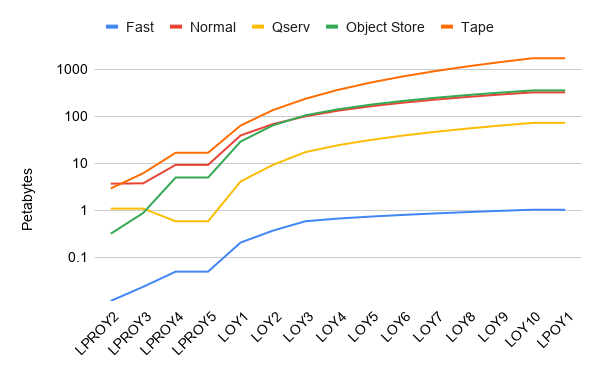
\includegraphics[width=0.8\textwidth]{figs/storage}
\end{center}
\caption{Evolution of {\bf cumulative} storage needs for Rubin Observatory. Details are given in the appendix. This plot shows the total storage needed at the \gls{USDF} of different types. Storage at other data facilities, including the Chilean data access center, are not included here. The \gls{USDF} is responsible for the last two years of pre operations (LPROY4-5) which are transition to \gls{USDF}, the survey years (LOY1-10), and the post operations years (only the first year of two is shown).\label{fig:storage}}
\end{figure}

There is an existing agreement with IN2P3 \citedsp{Agreement-51} to provision and execute 50\% of the total Data Release Production; the \gls{USDF} awardee will need to work with IN2P3 to enable this production.
It is incumbent upon the \gls{USDF}to develop and deploy systems for effectively managing split-site data processing.

Another facility may yet provide a further 25\% of processing power which would also have to be integrated in the model. If that happens, then the corresponding scope would be removed from the \gls{USDF}. For purposes of the \gls{FOA}, it can be assumed the \gls{USDF} will do 50\% of the Data Release Production.

The price of disk and tape media purchases over time have a profound effect on the \gls{USDF} budget over 10 years.
The FOA proposal should explicitly state the assumed pricing factors over the life of the survey for annual hardware purchases. It is assumed that the cost of media will decrease over time, and the annual decrements should be called out in the proposal (net of annual consumer inflation).


\tiny \begin{longtable} { |p{0.22\textwidth}  |r  |r  |r  |r  |r  |r  |r  |r  |r  |r  |r  |r |} 
\caption{On floor LDF storage estimates during Operations
 \label{tab:storageFloorOps}}\\ 
\hline 
\textbf{LDF Storage (on the floor)}&\textbf{unit}&\textbf{LOY1}&\textbf{LOY2}&\textbf{LOY3}&\textbf{LOY4}&\textbf{LOY5}&\textbf{LOY6}&\textbf{LOY7}&\textbf{LOY8}&\textbf{LOY9}&\textbf{LOY10} \\ \hline
{APDB}&{TB}&{24}&{24}&{24}&{24}&{24}&{24}&{24}&{24}&{24}&{24} \\ \hline
{Qserv Czar/ Object}&{TB}&{182}&{347}&{562}&{643}&{711}&{774}&{835}&{894}&{951}&{1006} \\ \hline
\textbf{Total Fast}&\textbf{TB}&\textbf{206}&\textbf{371}&\textbf{586}&\textbf{667}&\textbf{735}&\textbf{798}&\textbf{859}&\textbf{918}&\textbf{974}&\textbf{1029} \\ \hline
{Normal}&{TB}&{38983}&{67976}&{99538}&{131025}&{162321}&{193727}&{225288}&{256991}&{288788}&{320731} \\ \hline
{Qserv Storage}&{TB}&{4094}&{9257}&{17275}&{24144}&{31277}&{38734}&{46555}&{54716}&{63206}&{72017} \\ \hline
{LSSTCam Raw Images}&{TB}&{6982}&{11798}&{16614}&{21430}&{26246}&{31062}&{35878}&{40694}&{45510}&{50326} \\ \hline
{LSSTCam Output Images}&{TB}&{3933}&{10676}&{16857}&{23599}&{30342}&{37084}&{43827}&{50570}&{57312}&{64055} \\ \hline
{LSSTCam Output Coadd Images}&{TB}&{8636}&{16364}&{23182}&{23182}&{23182}&{23182}&{23182}&{23182}&{23182}&{23182} \\ \hline
{LSSTCam Output Parquet}&{TB}&{9302}&{25248}&{47839}&{71758}&{95678}&{119597}&{143516}&{167436}&{191355}&{215275} \\ \hline
{Object Store}&{TB}&{28854}&{64086}&{104491}&{139969}&{175447}&{210925}&{246403}&{281881}&{317359}&{352837} \\ \hline
{LSSTCam Raw Images}&{TB}&{6982}&{11798}&{16614}&{21430}&{26246}&{31062}&{35878}&{40694}&{45510}&{50326} \\ \hline
{All Data Products/ Backup}&{TB}&{47626}&{106967}&{194226}&{309242}&{451681}&{621564}&{818915}&{1043758}&{1296109}&{1575992} \\ \hline
{All Object Store-Only Products}&{TB}&{8636}&{16364}&{24091}&{31818}&{39545}&{47273}&{55000}&{62727}&{70455}&{78182} \\ \hline
{Tape}&{TB}&{63245}&{135129}&{234931}&{362490}&{517473}&{699899}&{909793}&{1147179}&{1412074}&{1704500} \\ \hline
\end{longtable} \normalsize

\tiny \begin{longtable} { |p{0.22\textwidth}  |r  |r  |r  |r  |r  |r  |r  |r  |r  |r  |r  |r |} 
\caption{Compute needs during Operations \label{tab:computeSizingOps}}\\ 
\hline 
\textbf{Data Release Production}&\textbf{units}&\textbf{LOY1}&\textbf{LOY2}&\textbf{LOY3}&\textbf{LOY4}&\textbf{LOY5}&\textbf{LOY6}&\textbf{LOY7}&\textbf{LOY8}&\textbf{LOY9}&\textbf{LOY10} \\ \hline
{LSSTCam visit input size}&{TB}&{1911}&{3822}&{5733}&{7644}&{9556}&{11467}&{13378}&{15289}&{17200}&{19111} \\ \hline
{DRP compute}&{core-hours}&{4.5E+07}&{8.2E+07}&{1.2E+08}&{1.6E+08}&{2.0E+08}&{2.5E+08}&{2.9E+08}&{3.3E+08}&{3.7E+08}&{4.1E+08} \\ \hline
{Alert Production}&{units}&{LOY1}&{LOY2}&{LOY3}&{LOY4}&{LOY5}&{LOY6}&{LOY7}&{LOY8}&{LOY9}&{LOY10} \\ \hline
{AP cores}&{cores}&{1,188}&{1,188}&{1,188}&{1,188}&{1,188}&{1,188}&{1,188}&{1,188}&{1,188}&{1,188} \\ \hline
{US DAC}&{units}&{LOY1}&{LOY2}&{LOY3}&{LOY4}&{LOY5}&{LOY6}&{LOY7}&{LOY8}&{LOY9}&{LOY10} \\ \hline
{LSP cores}&{cores}&{517}&{933}&{1,399}&{1,866}&{2,332}&{2,798}&{3,265}&{3,731}&{4,198}&{4,664} \\ \hline
{Qserv data per node}&{TB/ node}&{43}&{43}&{86}&{86}&{86}&{86}&{173}&{173}&{173}&{173} \\ \hline
{Qserv nodes}&{nodes}&{95}&{216}&{309}&{348}&{364}&{451}&{436}&{408}&{367}&{418} \\ \hline
{LSP cores/ science user}&{cores/ user}&{0.1}&{0.2}&{0.2}&{0.2}&{0.3}&{0.4}&{0.4}&{0.5}&{0.6}&{0.6} \\ \hline
{Chilean DAC}&{units}&{LOY1}&{LOY2}&{LOY3}&{LOY4}&{LOY5}&{LOY6}&{LOY7}&{LOY8}&{LOY9}&{LOY10} \\ \hline
{LSP cores}&{cores}&{103}&{187}&{280}&{373}&{466}&{560}&{653}&{746}&{840}&{933} \\ \hline
{Qserv nodes}&{nodes}&{95}&{216}&{309}&{348}&{364}&{451}&{436}&{408}&{367}&{418} \\ \hline
{Staff LSP}&{units}&{LOY1}&{LOY2}&{LOY3}&{LOY4}&{LOY5}&{LOY6}&{LOY7}&{LOY8}&{LOY9}&{LOY10} \\ \hline
{LSP cores}&{cores}&{52}&{93}&{140}&{187}&{233}&{280}&{326}&{373}&{420}&{466} \\ \hline
\end{longtable} \normalsize



\newreqtype{INFR}
\reqsimp{}{}{}{}{}
{
The cost model for work package \ref{sect:wp01} shall include the nonlabor
costs to purchase computing hardware meeting the operation needs of the Rubin Observatory \gls{US} Data Facility as summarized in \tabref{tab:storageFloorOps}, \tabref{tab:computeSizingOps}, and \figref{fig:prodinfra}.
}

\reqsimp{}{}{}{}{}
{
The cost model for work package \ref{sect:wp01} shall include the labor costs to
manage and operate the computing for the  Rubin Observatory \gls{US} Data Facility.
}

The infrastructure team will oversee and manage the Data Facilities'
performance and strategy. The \gls{USDF} infrastructure team will
instantiate and operate a combination of hardware and software as
services, including problem management, incident management, request
response, and installing and validating changes in conjunction with
the IT change control process. This includes maintenance of
configuration information at the service level, e.g., an application
map showing the reliance of the service on all software and ITC, being
aware of security configurations and other operational matters, and
handling both network security and authorization infrastructure, and
operational security associated with network-based security.

\reqsimp{}{}{}{}{} { The awardee shall integrate staff in the Rubin
  infrastructure team from \gls{IN2P3}. It is assumed that any
  additional data facility involved in \gls{DRP} will also integrate
  staff into this team. }

\reqsimp{}{}{}{}{}{}
{
The USDF shall have a high availability architecture including: automated monitoring of services, including alerts to Rubin engineers about degraded service,   redundancy of service,
the capability to upgrade infrastructure in a rolling fashion to minimize outages, and (preferably) automated ejection of mis-behaving infrastructure elements from the resource pool.
}

\reqsimp{}{}{}{}{} {The facility shall have no more than a total of three days of
unplanned downtime per year. }

\reqsimp{}{}{}{}{} { The facility shall schedule planned downtimes only after consultation with Rubin
and shall provide a service level agreement for the facility with ticket turnaround
times, etc.}

\reqsimp{}{}{}{}{}{}
{The facility  shall provide access to logs or a logging service (e.g., Kibana or Splunk) to any infrastructure services that may be affecting Rubin systems. This potentially means access to Kubernetes or storage host logs. \label{req:logs}}


\subsection{Security} \label{sec:sec}
The provider shall be responsible for the security of the infrastructure and keep that infrastructure patched and configured according to security best practices, including regular security testing and remediation of any high-severity findings.

Rubin Observatory  expects to have thousands of users in America and beyond. Facility security polices should not prevent direct internet access to our public-facing services from registered and unregistered (as appropriate) users (e.g., by mandating VPN-only access see \reqref{req:novpn}).

Rubin already has a data base of users and uses CI-Login for federated Authentication, facility security policies should allow Rubin to or someone we contracted with, to manage user authentication and to our services. (See also \reqref{req:cil}.

Rubin requires the right to reject any security policy that would require us to permit decryption of TLS traffic to the infrastructure provider or third parties e.g., to network filtering appliances.

Facility  security policies  must allow authorized administrators from Rubin Observatory to investigate errors and debug technical issues on kubernetes nodes or other service hosts. (See also \reqref{req:2fa} \reqref{req:logs}.)

\reqsimp{}{}{}{}{}{}
{
Rubin has many SSL certificates and has many domains registered facilities should  allow Rubin to continue  managing SSL certificates,  using our own domain registrar and  deploying public-facing services under our own domains (e.g., lsst.io) and with an external DNS service (e.g., Amazon’s Route53)
}
\reqsimp{}{}{}{}{}{}
{
The provider shall be responsible for the security of the infrastructure and keep that infrastructure patched and configured according to security best practices, including regular security testing and remediation of any high-severity findings.
}
\reqsimp{}{}{}{}{}{}
{
	Administrative access to the infrastructure shall require two-factor authentication. \label{req:2fa}
}


\subsection{Science Platform}
\reqsimp{}{}{}{}{} {The facility shall support federated login for the \gls{LSP}
such as \gls{CI}-Logon. \label{req:cil}}

\reqsimp{}{}{}{}{} {The facility shall support access to the \gls{LSP} services from
unrestricted IP address - i.e. not requiring a \gls{VPN}. \label{req:novpn}}
\\ Some services may not require authentication.

\reqsimp{}{}{}{}{} { The facility shall support and demonstrate knowledge of the data
production deployment mechanisms e.g. Helm, ArgoCD, Kubernetes and Puppet.
}

Any facility should consider that the Science Platform is a
continuously deployed system that exposes shell access and ad-hoc
capabilities to users and the data center resources as a platform to
developers. So it is a poor fit to more “buttoned-down” data center
models. Rolling upgrades should also be standard to allow for less
downtime. There is significant redundancy in the system to allow for this.


\subsubsection{Kubernetes}\label{sec:k8s}
Specifically concerning K8S there are several requirements to be considered.
\reqsimp{}{}{}{}{}{}
{
 The facility shall provide  Managed Kubernetes, including all necessary administrative access to create/destroy/administer clusters and debug pod and storage problems, no more than one minor version behind current (e.g. if current is 1.18, 1.17 is required).
	See for example \citeds{DMTN-136} \label{req:k8s}	}

\reqsimp{}{}{}{}{}{}
{
The facility shall provide self serve tools for machine and cluster management. e.g. K8S admin.
}
\reqsimp{}{}{}{}{}{}
{
USDF self serve tools shall include command-line access to any managed services  through Unix/Linux systems. Command-line access (via an API, for example) to be available to engineers in addition to any web-console access.
}

\reqsimp{}{}{}{}{}{}
{
The facility shall provide ability for Rubin engineers to solely or jointly  manage ingress services to the Kubernetes cluster(s)
}
\reqsimp{}{}{}{}{}{}
{
The facility shall provide the ability for Rubin services to utilize Kubernetes Dynamic Volume Provisioning.
}
\reqsimp{}{}{}{}{}{}
{
 The facility shall enable storage to be  exposed as a POSIX filesystem to our services  permitting exclusive file locks as well as lock reservations (e.g. NFSv4 or NFS v.3 with the ability to specify/configure lock daemon behavior). \label{req:posix}
}

\reqsimp{}{}{}{}{}{}
{
The facility shall allow Rubin services to control UID/GID of users in the POSIX filesystem (see \reqref{req:posix}).
}

\reqsimp{}{}{}{}{}{}
{
The facility shall allow select services pods (not users) to access storage with escalated privileges
}

See also \secref{sec:networking}.



\subsection{Alerts}
\label{sec:alerts}

As a part of regular operations, the project will scan all images taken by the
\gls{LSST} Camera for transient and variable sources, announcing results to the
scientific community within 60\,s of the data being taken through an alert stream
provided to a set of preselected community alert brokers.
\citeds{LDM-612} provides an overview of the Rubin Observatory alert system.

The external ``community brokers'' will receive the
full alert stream generated by Rubin Observatory, and bear the primary
responsibility of redistributing relevant alerts to science users. Rubin
will generate up to 10 million alerts per night, with the average
alert packet size being 82\,\gls{KB} (see \reqref{req:netbroker}).

The current system architecture locates all scientific processing
pipelines, including those used to identify transients and variables
(the ``Alert Generation Pipeline''), at the \gls{USDF}.
Each exposure corresponds to around 8.2\,GB of raw data,
which must be shipped with extremely low latency over the dedicated \gls{LHN} to
the \gls{USDF} to enable the Alert Generation Pipeline to execute and
deliver the results to the community alert brokers within the allocated time window (see
\reqref{req:netlat}).

Increased bandwidth allocation from the Data Facility would provide an opportunity
to increase the number of community brokers supported.


\reqsimp{}{}{}{}{} {The USDF shall host an specific dedicated cluster for
prompt processing as defined in \citeds{LDM-151}. See also \appref{sec:prompproc}.
\label{req:alerts}}

One could discuss this as a service level rather than dedicated resources.

\reqsimp{}{}{}{}{} {The USDF shall support Kafka\footnote{\url{https://kafka.apache.org/}} for alert distribution.
\label{req:alertdist}}

\subsection {Solar system object processing}

During the 24 hours following the completion of an observing night, the Solar System Processing Pipeline will be executed to carry out real-time identification of objects within our solar system.
This procedure relies on knowledge of all previously detected solar system objects.
The \gls{MPC} maintains such a catalog; Rubin will ingest the latest version of this catalog every evening and orbits will be computed using all available data, not only Rubin observations.
Resultant new identifications and associations will be transmitted publicly in the
event alert stream; candidate discoveries are sent to the \gls{MPC} for inclusion
in the next night's catalog.

\reqsimp{}{}{}{}{}
{
The facility shall interface with the \gls{MPC}
both to ingest updated catalogs, and to transmit Rubin Observatory candidate discoveries, as part of the regular daily operations cycle.
}

Full details of the Solar System Processing Pipeline can be found in \citeds{LDM-156} and \citeds{DMTN-087}.

\subsection { Batch Computing}
The computing model in \tabref{tab:computeSizingOps} assumes two major processes along side \gls{LSP} usage: the alerts (see \reqref{req:alerts} and DRP.

\reqsimp{}{}{}{}{}
{
The USDF shall provide a batch processing system that integrates with the
Rubin Observatory Middleware to run the release processing. \label{req:drp}
}

\citeds{DMTN-123} describes the batch processing in detail - the baseline
for this will be Condor and Postgres (for the registry). The middleware is
ready to use an Object Store back end which will greatly facilitate job
distribution (see also \secref{sec:studies}).

\reqsimp{}{}{}{}{}
{
The USDF shall reserve about 10\% of processing for user jobs - this may be provided by the same batch system in place for \reqref{req:drp}. Or they could use a simpler system.
}

\reqsimp{}{}{}{}{}
{
The USDF shall provide monitoring tools for the batch processing to allow tracing of problems, restarting of jobs, etc.
}



\subsection{Databases} \label{sec:dbs}

The USDF will need to host several databases (see also \citeds{DMTN-104}:

\begin{itemize}
\item Managed Consolidated Database - general-purpose relational database management
that supports other services. It includes metadata and provenance, but
it does not include the large catalog science data products that are
generated as files and loaded into the Qserv parallel distributed
database. This should be Postgres.

\item LSP Database - mainly for user data and meta information about the system. This is currently Postgres
\item \gls{EFD} (Cache) - Engineering data is stored in an Influx database. A copy may need to be hosted near the Science Platform and some high level (averaged) values may need to be stored in a a relational system such
as the consolidated database.
\item \gls{APDB} - Performance critical internal database used to support Alert Production; will not support end- user queries.  See also \citeds{DMTN-018}.
\end{itemize}




\subsection {Bulk Download}
\label{sec:bulk}

Rubin Observatory \gls{USDF} will support transfer of the full dataset, or
large subsets, to data centers in the US and other countries, subject to future agreements.
The \gls{USDF} may also support bulk downloads to  scientific collaborations which wish to perform additional systematic processing (e.g., shift-and-stack image analysis to search for outer Solar System objects).

\reqsimp{}{}{}{}{}
{
The USDF  shall provide a bulk download service, with concomitant implications for external bandwidth from Rubin storage to the public and research Internets, as well as for the provision of a storage management layer that facilitates reliable incremental export (e.g., \gls{Rucio}).
}

Some or all costs for bulk downloads may be borne by the users.

\subsection{Other Services}
There are other services outlined in construction to run at the \gls{USDF}.

\reqsimp{}{}{}{}{}
{
	Prospective Awardees shall enumerate the construction requirements listed in \appref{sec:dmsrreqs}
	derived from  \citeds{DMTN-104} and ensure they are covered.
 \citeds{LDM-129} provides a set of services covering these which could be considered (or alternatives suggested). The other services are shown in \figref{fig:prodinfra} and enumerated in \citeds{DMTN-104}.
 \label{req:otherservs}
}\\

The important point here is to cover the requirements not necessarily the services list.

\begin{figure}
	\begin{center}
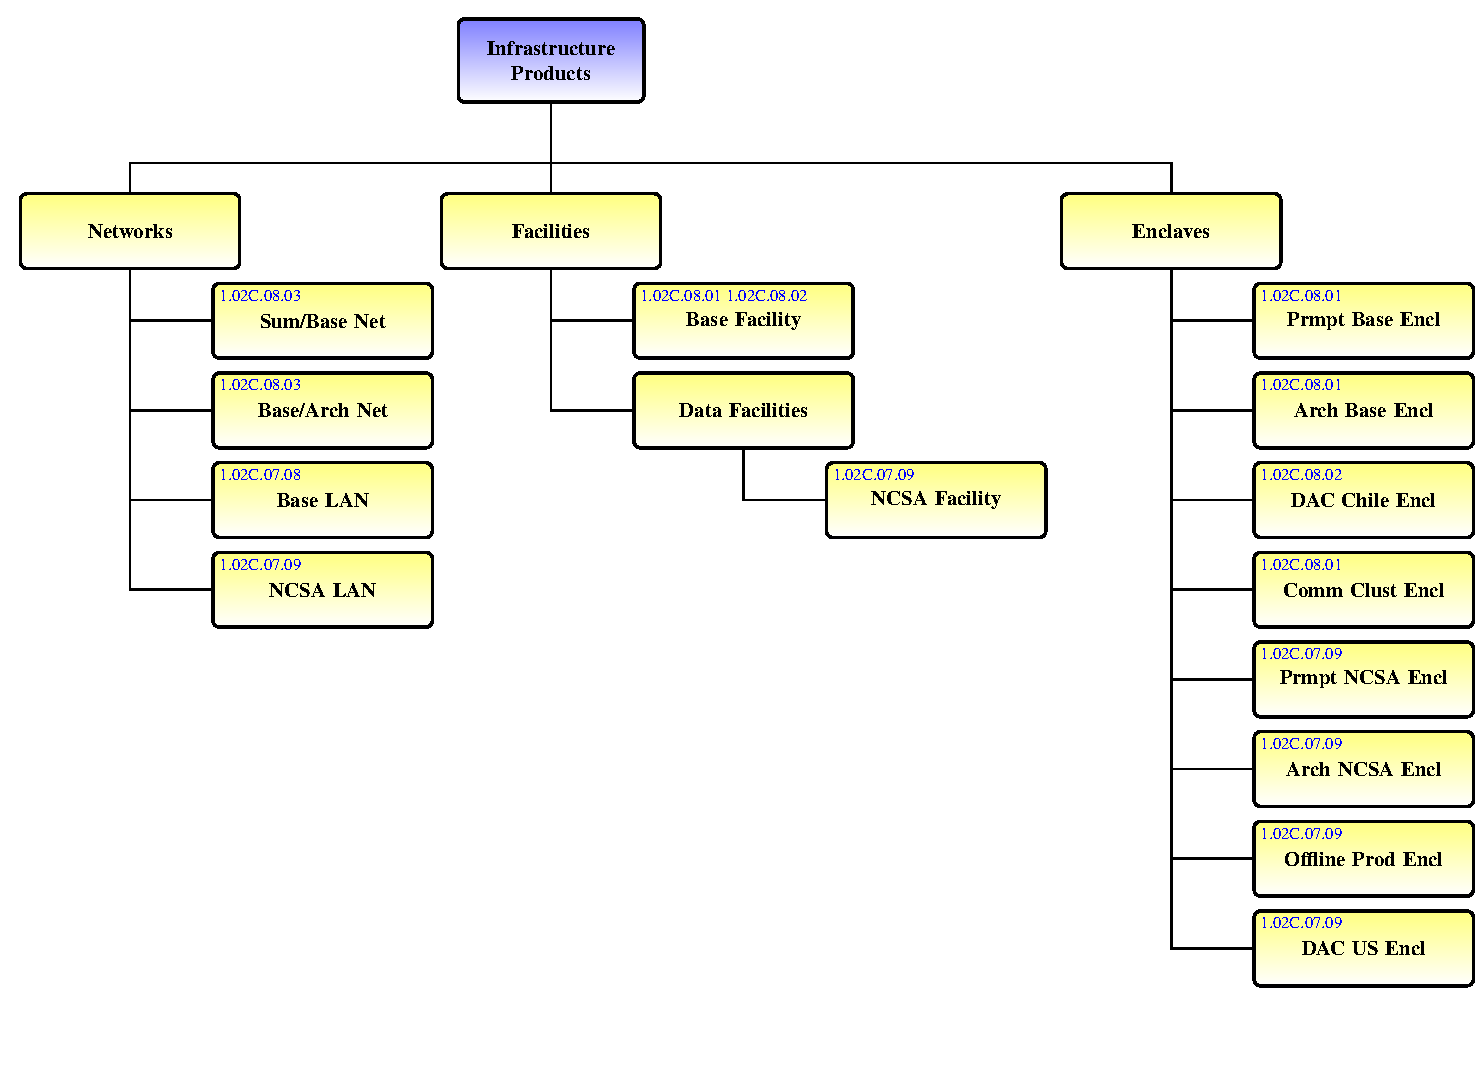
\includegraphics[width=0.9\textwidth]{figs/Main_INFRA}
	\end{center}
	\caption{Subset of the product tree from \citeds{DMTN-104} pertaining to Infrastructure \label{fig:prodinfra}}
\end{figure}

\subsubsection{Data transfer and preservation}
Within the services mentioned in \reqref{req:otherservs} there are a set of services concerning data
transfer, preservation and tracking. These bear particular scrutiny.

\reqsimp{}{}{}{}{}
{
 Prospective awardees shall transfer data from Chile. This data shall be archived, tracked and made
 available to Rubin processing systems.  See specifically \secref{sec:dbb}
}\\

Butler currently keeps track of files in Postgres and can be used with filesystems or S3.
S3 seems more scalable long term. See also \reqref{req:butler}

\reqsimp{}{}{}{}{}
{
 Image data shall be ingested into the Rubin butler. Files shall be accessible via an
 S3 compliant object store interface.
}\\

\reqsimp{}{}{}{}{}{}
{
	The facility  should provide a Postgres like database service for the Butler metadata.
	This service shall allow Rubin to  select extensions like PGSphere.
	It shall by performant for databases up to 100 TB.
	}

\reqsimp{}{}{}{}{}{}
{
	Any data services provided (filesystems, object stores, databases) shall be regularly backed up for disaster recovery, unless otherwise specified (e.g., /scratch).
}\\\\


These services are currently known  as Data backbone (DBB) - these could be installed/ported.





\subsection{\textbf{WP-02}: Rubin \gls{middleware} }
\label{sect:wp02}
The Rubin \gls{middleware} team acts as a center of general software development expertise to the Data Production department. Specific duties are:
\begin{itemize}
	\item Maintain and evolve \gls{middleware} which provides hardware and I/O abstractions for us in science and user codes.
	\item Maintain and evolve the \gls{Qserv} distributed database.
	\item Coordinate software build and release activities across the Data Production department.
	\item Conduct investigations into underlying technological and/or infrastructural changes (for example, potential migration of some or all services to commodity cloud infrastructure).
\end{itemize}

\newreqtype{MDLW}
\reqsimp{}{}{}{}{}
{
The facility shall support the \gls{middleware} team preferably by integrating staff in the team which is
under direct Rubin management.
}

\reqsimp{}{}{}{}{}
{
Within the middleware team the facility shall assist with integration of the Gen3 butler and other middleware.
}

\reqsimp{}{}{}{}{}
{
Within the middleware team the facility shall assist with integration of the task framework with local processing framework such as HTCondor. See also \citedsp{LDM-152}  and \citedsp{DMTN-123}. As noted in \secref{sect:wp01} processing will also take place in IN2P3.
}\\
Workflow is an area potentially requiring significant some work to deploy in a new operations \gls{USDF}. This could be outsourced from the \gls{USDF} -
other groups are expert in workflow and could be useful.

\reqsimp{}{}{}{}{}
{
	The butler requires a meta data database for which a Postgres installation is required. See also \secref{sec:dbs}. \label{req:butler}
}

\subsection{\textbf{WP-03}: Rubin Execution}
\label{sect:wp03}
The Rubin execution team requires some level of support at the data facility.
The Execution team will run the pipelines which generate prompt and data release products for the community, as well as \gls{calibration}, environmental, quality and \gls{metadata} products for the data production and system performance departments.
There may be a need to run services to satisfy specific use cases as yet unidentified.
Execution staff at the \gls{USDF} will integrate reusable services, data layer, software, services provided by MoU, and \gls{ITC} to produce functioning 
services.

\newreqtype{EXEC}
\reqsimp{}{}{}{}{}
{
The awardee shall integrate staff in the Rubin execution team which 
already has members from \gls{SLAC} and
 \gls{IN2P3}. It is assumed any additional data facility involved in \gls{DRP} 
will also integrate staff in this team.
}




\section{Project Management}

The Rubin Operations plan details the operational organization. An abbreviated
description of the Rubin System is given in the document
``Vera C. Rubin Observatory System and Organization Description''
attached to the \gls{FOA}.

The \gls{USDF} is part of the Data Production department.
The department is built on teams as
depicted in \figref{fig:orgchart}. Most \gls{USDF} staff will be in the
Infrastructure team, with several in middleware and execution. These teams will have leads that report to the Associate Director for Data Production. The \gls{USDF} Infrastructure lead will be a staff member of the \gls{USDF}. The other DP
team leads are based at SLAC or NOIRLab.

It is essential that the Data Facility, whatever its host institution,
integrates with this Operations structure; see the attached description
for more details.
In particular, we emphasize that although Rubin staff are spread across multiple groups and multiple institutions, they are expected to collaborate as members of a single functional organization, working together across institutional boundaries to achieve the best outcomes for the project. This organization can be
described as a mini-matrix in Data Production. See the attached description document, section 4, Figure 8. The USDF will have an administrative structure of
its own with a point of contact that will provide advice and input to the
AD for Data Production along with similar individuals from other
data centers (see also \reqref{req:spoc} below).

\begin{figure}
\begin{center}
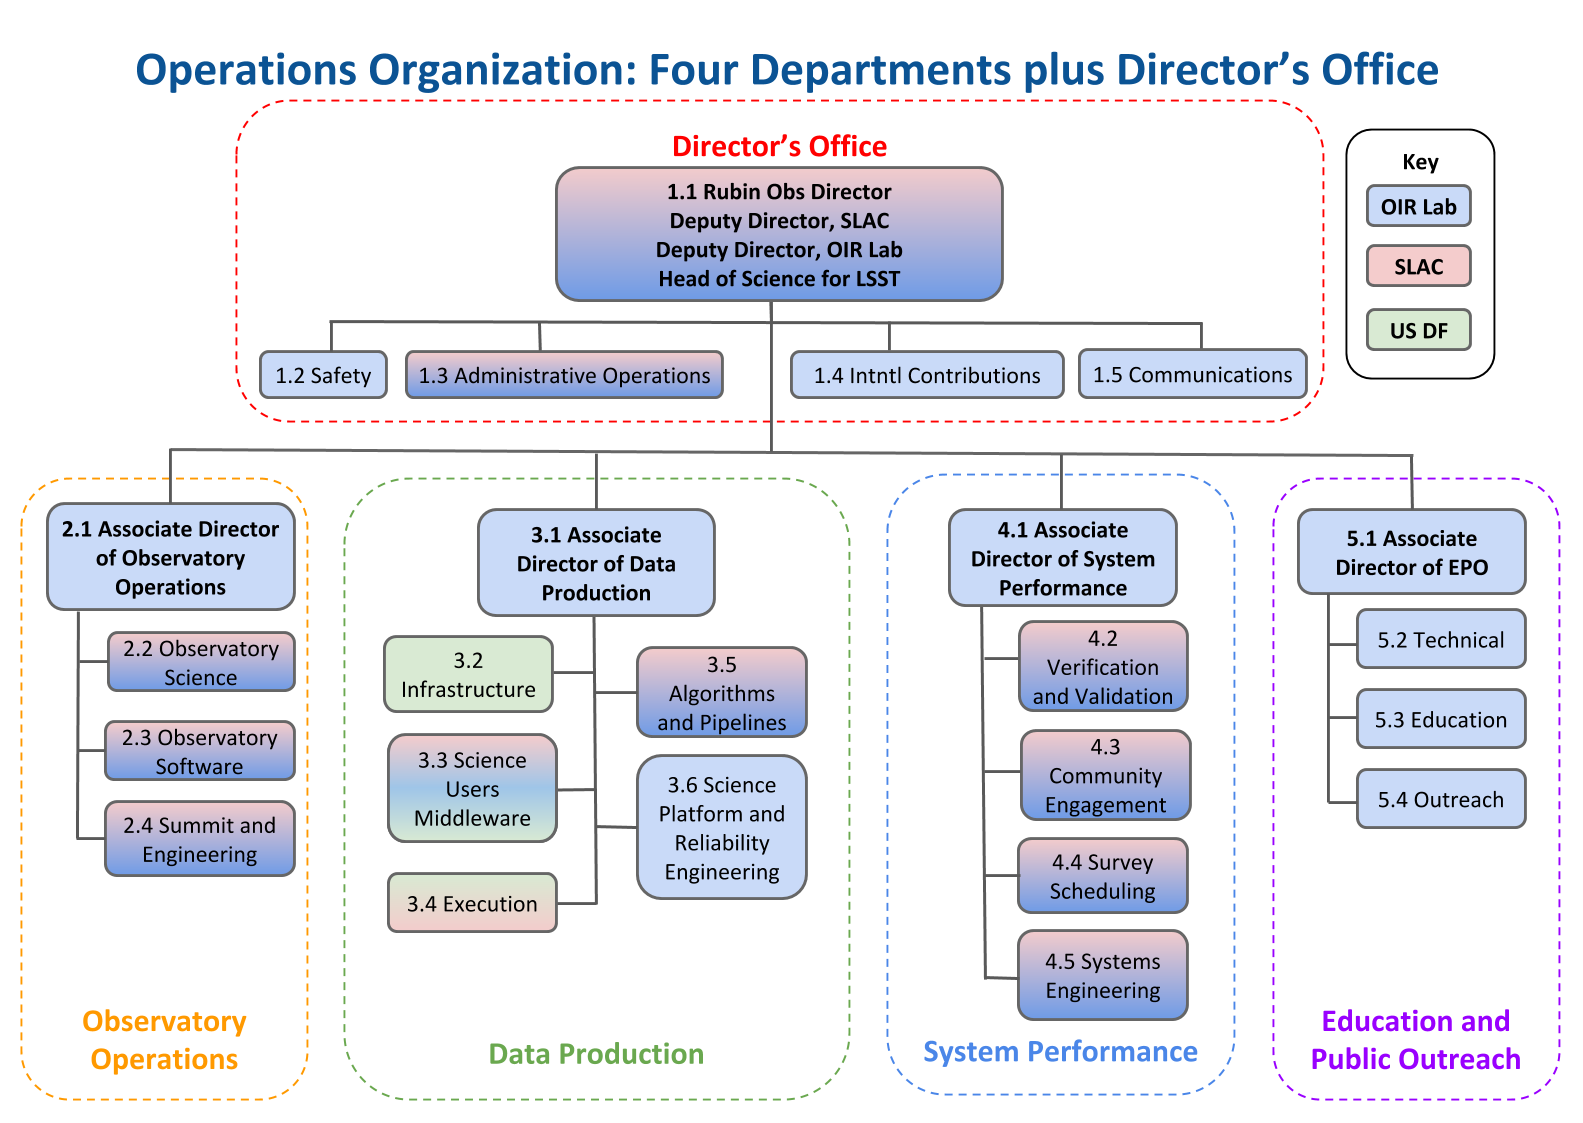
\includegraphics[width=0.8\textwidth]{figs/orgchart}
\end{center}
\caption{
The Vera Rubin Observatory Organization Chart. Shaded boxes indicate shared staff across operations partners. Staff at affiliate institutions  are included within their associated operations partner (i.e. not separately).
\label{fig:orgchart}}
\end{figure}

\newreqtype{MNGT}
\subsection{Management}\label{sec:manage}

\reqsimp{}{}{}{}{}
{
There  shall be  a the single point of contact for all managerial
aspects of the work. \label{req:spoc}
}

\reqsimp{}{}{}{}{}
{
  This work shall be carried out within the Rubin Observatory management structure under the Data Production
  department.
}

\reqsimp{}{}{}{}{}
{
The awardee shall inform Rubin Observatory management of planned changes in the
availability of staff in support of the work.
}

\reqsimp{}{}{}{}{}
{
The awardee shall conform to Rubin Observatory management practices
including use of tracking and reporting tools adopted by the observatory.
\citeds{DMTN-020} is an example of construction era practices.
}
\reqsimp{}{}{}{}{}
{The awardee will support Rubin management in all oversight committee meetings, joint agency reviews, and other management body activities as deemed necessary or desired by AURA and SLAC. 
} 

\newreqtype{PERF}
\subsection{Performance}\label{sec:perf}
\reqsimp{}{}{}{}{}
{
The awardee shall be responsible to Rubin Observatory management organizations AURA and SLAC for performance of the activities and capabilities detailed in this
SOW through a negotiated set of performance metrics. 
}
\reqsimp{}{}{}{}{}
{
The awardee's staff will receive annual performance input from Rubin management to be included in the awardee annual performance assessment process.
}

\reqsimp{}{}{}{}{}
{
Rubin management will have the authority to request that awardee staff who under perform be replaced.
}

\newreqtype{REPT}
\subsection{Reporting}
\reqsimp{}{}{}{}{}
{
The awardee shall provide a regular progress report on the status of
activities, support provided, status of anomaly investigations, etc. This
report shall cover all WPs described in this statement of and shall include
contributions from sub-contractors as appropriate. This may be integrated in
a more general Rubin Observatory report. DOE may place other, independent,
reporting requirements on the awardee.
}

\reqsimp{}{}{}{}{}
{
The frequency of reporting shall be monthly, quarterly, and annual, as
appropriate.
}

\reqsimp{}{}{}{}{}
{
Monthly reporting shall include SLA metrics to be agreed with Rubin Observatory
such as cumulative downtime, issue turn around time etc.
}

\newreqtype{COMS}
\subsection{Communications}
Regardless of funding streams, Rubin Observatory \gls{Operations} should function as one project.
While we recognize that this is not always easy for staff already embedded in another institution, it is important that we share the same tools to avoid silos and to communicate effectively about our work and to our communities.
The three primary platforms for communication at Rubin are the \gls{JIRA} ticketing system, the Slack chat system, and the web forum, community.lsst.org. Technotes are produced via LSST the Docs \citedsp{sqr-006} for Data Production. Official documentation is placed in Docushare and we also heavily use confluence. We would expect that Data Facility team members would engage with all of these.

An important part of both LSST Construction and Operations will be writing and sharing code.
All software written for \gls{LSST} is open source and publicly available, and is developed following the workflows and engineering standards described in the LSST Developer guide at \url{developer.lsst.io}.
Code developed at institutions must be developed and made available under the same conditions.


\reqsimp{}{}{}{}{}
{
\gls{USDF} staff shall use the Rubin Observatory communication tools such as JIRA, Slack and LSST the Docs.
}
\reqsimp{}{}{}{}{}
{
Any code developed for the Rubin Observatory Project shall be developed in the project repository (currently github) and shall carry the project open source license (currently \gls{GPL}).
}


\newreqtype{TRVL}
\subsection{Meetings and Travel}

\reqsimp{}{}{}{}{}
{
The awardee shall support  teleconferences  and travel in support of the
above work packages as required and agreed by both parties. At a minimum this
would include weekly video calls and in person meetings two times per year.
}

\reqsimp{}{}{}{}{}
{
The awardee shall participate in the NET group and attend the monthly telecons and meetings once or twice a year
as needed.\footnote{\url{https://confluence.lsstcorp.org/pages/viewpage.action?pageId=20284335}}
}

\newreqtype{DLVR}
\section{Deliverables}

\reqsimp{}{}{}{}{}
{
Any code deliverables shall adhere to the standards and guidelines of
Rubin Observatory as on \url{developer.lsst.io}
}



\section{Data Management System portability and cloud computing}
\label{sec:studies}

Although the project baseline has physical compute facilities in Chile and \gls{USDF}, with split-site processing at \gls{IN2P3}, we have designed the system to be flexible with regard to the environment within which it is deployed.
It is also possible the computing systems at the \gls{USDF} and Chilean Access Centers will not satisfy the entire demand for near-the-data processing and peak load; computing models that allow externally-funded resources to be easily and efficiently used are desirable.
Public clouds, by handling the accounting and resource management for multi-tenancy, provide an interesting solution for this, provided that potentially-large data storage costs can be mitigated. Any \gls{USDF} partner shall be open to continuing investigations and partnerships of this type in collaboration with
Rubin Observatory.

In this vein, we have recently undertaken studies to investigate the possibility of performing \gls{LSST} data processing on cloud computing platforms provided by both Google and Amazon.
On the Google cloud platform, we demonstrated that several of the major components of the \gls{Data Management System} could be run effectively.
In particular,

\begin{itemize}

  \item{we deployed the \gls{Qserv} database system, demonstrating that it could achieve 80\% of the performance we achieved in-house on physical hardware;}

  \item{we demonstrated data transfer adequate for \gls{Prompt Processing}, within the limits of the current \gls{LHN} networks available for testing;}.

  \item{we deployed and tested the Prompt Products Database;}

  \item{we deployed an instance of the \gls{LSP}.}

\end{itemize}

Note that the \gls{LSP} in particular is engineered around the \gls{K8S} system (\secref{sec:k8s}), and therefore deploys extremely smoothly to the Google Cloud.
The results of this study are described in detail in \citeds{DMTN-125}.

The Google study did not investigate the single largest compute load that the \gls{LSST} will face: \gls{Data Release Processing}.
We are now addressing this on Amazon Web Services / Elastic Compute Cloud, as described in \citeds{DMTN-114}.
This work is ongoing at time of writing; initial results are positive.

We believe that these studies demonstrate the flexibility of the \gls{DM} System to a variety of deployment environments, and particularly illustrate the value --- and importance to the project of --- \gls{K8S}.

\appendix
\section{Sizing details} \label{sec:sizeinputs}

The following simplified sizing may be used to give the input sizes for a
cost model.
The storage sizes are given in \tabref{tab:storageFloorOps}
while the compute is given in \tabref{tab:drpAndAlertSizing}
and \tabref{tab:lspSizing}. The cumulative storage requirements are also shown
in \figref{fig:storage}. The cumulative processing required is shown below
in \figref{fig:cores}.

\begin{figure}
\begin{center}
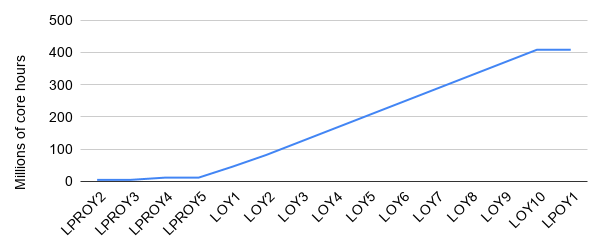
\includegraphics[width=0.8\textwidth]{figs/cores}
\end{center}
\caption{Evolution of {\bf cumulative} computing needs for Rubin Observatory. Details are given below. Compute at other data facilities, is not included here. The \gls{USDF} is responsible for the last two years of pre operations (LPROY4-5) which are transition to \gls{USDF}, the survey years (LOY1-10), and the post operations years (only the first year of two is shown).\label{fig:cores}}
\end{figure}

Some useful inputs are provided in \tabref{tab:Inputs}.

\tiny \begin{longtable} { |p{0.22\textwidth}  |r  |r  |r  |r  |r  |r |} 
\caption{Various inputs for deriving costs - 2019 represents current holdings. \label{tab:Inputs}}\\ 
\hline 
\textbf{Year}&\textbf{2019}&\textbf{2020}&\textbf{2021}&\textbf{2022}&\textbf{2023} \\ \hline
{Core-hours Needed Total (DRP)}&{}&{4.41E+06}&{4.41E+06}&{1.12E+07}&{4.53E+07} \\ \hline
{Annual Increase}&{}&{4.41E+06}&{0.00E+00}&{6.81E+06}&{3.40E+07} \\ \hline
{Time to Process days}&{}&{100.0}&{100.0}&{100.0}&{200} \\ \hline
{Time to Process hours}&{}&{2,400}&{2,400}&{2,400}&{4,800} \\ \hline
{Instantaneous cores (DRP) Total}&{}&{1,836}&{1,836}&{4,673}&{9,430} \\ \hline
{Instantaneous cores (DRP) Annual increase}&{1152}&{1,836}&{0}&{2,837}&{7,093} \\ \hline
{Instantaneous cores (Alerts)}&{}&{0}&{0}&{1188}&{1188} \\ \hline
{Cores (Alerts) Annual increase}&{}&{0}&{0}&{1188}&{0} \\ \hline
{Instantaneous cores (US DAC/ Staff)}&{540}&{540}&{540}&{141}&{568} \\ \hline
{Cores (US DAC/ Staff) Annual increase}&{}&{0}&{0}&{0}&{428} \\ \hline
{Instantaneous cores (Chilean DAC)}&{}&{0}&{0}&{26}&{103} \\ \hline
{Cores (Chilean DAC) Annual increase}&{}&{0}&{0}&{26}&{78} \\ \hline
{Qserv nodes (US DAC/ Staff)}&{}&{}&{}&{14}&{95} \\ \hline
{Qserv nodes (US DAC/ Staff) Annual Increase}&{}&{}&{}&{14}&{81} \\ \hline
{Qserv nodes (Chilean DAC)}&{}&{}&{}&{14}&{95} \\ \hline
{Qserv nodes (Chilean DAC) Annual Increase}&{}&{}&{}&{14}&{81} \\ \hline
\textbf{Total Cores Annual Increase}&\textbf{}&\textbf{1,836}&\textbf{0}&\textbf{4,051}&\textbf{7,599} \\ \hline
{Fast Storage (TB)}&{}&{12}&{24}&{50}&{206} \\ \hline
{Annual Increase (Fast)}&{}&{12}&{12}&{26}&{156} \\ \hline
{Normal Storage (TB)}&{3000}&{3680}&{3748}&{9241}&{38983} \\ \hline
{Annual Increase (Normal)}&{}&{680}&{68}&{5494}&{29742} \\ \hline
{Latent Storage  (TB)}&{}&{319}&{876}&{4966}&{28854} \\ \hline
{Annual Increase (Latent)}&{}&{319}&{557}&{4090}&{23888} \\ \hline
{High Latency (TB)}&{}&{2910}&{6128}&{16733}&{63245} \\ \hline
{Annual Increase (High Latency)}&{}&{2910}&{3218}&{10605}&{46512} \\ \hline
{Chilean DAC Fast Storage (TB)}&{}&{}&{}&{}&{156} \\ \hline
{Annual Increase (Fast Chilean DAC)}&{}&{}&{}&{}&{156} \\ \hline
{Chilean DAC Latent Storage (TB)}&{}&{}&{}&{}&{28854} \\ \hline
{Annual Increase (Latent Chilean DAC)}&{}&{}&{}&{}&{28854} \\ \hline
{Annual price decrease CPU}&{}&{10\%}&{}&{}&{} \\ \hline
{Annual price decrease Storage}&{}&{5\%}&{}&{}&{} \\ \hline
{Annual price decrease Qserv}&{}&{8\%}&{}&{}&{} \\ \hline
\end{longtable} \normalsize


\subsection{Processing Plan}

This model assumes the following processing:
\begin{itemize}
\item Precursor data (HSC RC2 and a similarly-sized DESC DC2 subset) is reprocessed each month during the Construction period using the Data Release Production (DRP).
\item A large precursor reprocessing of HSC PDR2 (or equivalent) is completed twice a year.
Products from one of these reprocessings will be released as Data Preview 0 (DP0) by the operations team. This will not be done at the \gls{USDF}.
\item One or more of these processings will be devoted to ComCam and LSSTCam science data during Commissioning. Some processing at the \gls{USDF} might occur in the
transition in late FY22. If not then, certainly in FY23 in advance of full operations. ComCam data will be released as DP1. LSSTCam commissioning data will be released as DP2 soon {\it after} the start of full operations in FY24.
\item Alert Production (AP) processing happens continuously as LSSTCam science images are obtained.
AP hardware is purchased in FY23 to support this.
\item DR1 processing begins after the first 6~months of the survey; the hardware for this can be part of the purchase during FY23.
\item Annual DRP execution starts at the beginning of LSST Operations Year 2 with the processing for DR2.
The hardware for each year's processing must be purchased and ready for use at the beginning of the year, so it is allocated in the tables to the prior fiscal year, when the images for that processing were taken.

\end{itemize}

Some storage for raw data needs to be in place at the beginning of the fiscal
year, but it can be ramped up over the course of the year.
As a simplification it is allocated to the fiscal year in which it will be used.

\subsection{Operations Storage Model}

\subsubsection{Overview}

Values are computed for the amount of storage expected to be "on the floor" at the beginning of each fiscal.
Key scientific and algorithmic assumptions made include:
\begin{itemize}
\item All significant intermediates and data products generated by Data Release Production processing need to be kept on filesystem disk until the DRP is complete.
Some scratch space is provided to hold small, temporary intermediates.
If some intermediates could be removed during DRP when it is known they will no longer be needed, some space savings could be realized.
\item HSC RC2 processing is representative of the outputs that DRP will generate (see e.g. PDR2\footnote{https://hsc-release.mtk.nao.ac.jp/doc/index.php/sample-page/pdr2/}
The coadd storage is doubled to account for an additional "good-seeing" coadd along with the existing "deep" coadd.
\item Processed visit images (PVIs) and catalogs in Parquet format start on "normal" filesystem disk but then move to object storage at the completion of the DRP, with lossy compression of the PVIs at that time.
This is in accordance with \jira{RFC-325}, although the relevant LCR has not yet been approved.
Object storage is expected to be cheaper and more scalable for read-only data products; filesystem storage is used for data that is being generated or modified.
\item Raw images and coadd images are only temporarily stored on filesystem disk and are then rapidly moved to object storage, where they are retained.
\item Intermediates like warped images for coaddition are not survey data products and do not need to be kept beyond the end of the DRP and subsequent QA.
\end{itemize}

All data is backed up to tape permanently, including annual snapshots of filesystems.
Any incremental backups are assumed to be reusable or otherwise purged and hence not significant.

\subsubsection{Parameters}

The numbers of science users are estimates, using "Stack Club" users and Commissioning users for FY20 and 2021, followed by US science users in FY22 and FY23 for Data Preview data.
The bulk of US science users are not expected to arrive until after Data Release~1 at the beginning of LOY2.

Storage per science user is estimated based on today's usage at NCSA, scaled up as users become more active, and approaching the number given in \citeds{LSE-81} as Operations begins.
Note that it is expected that there will be a wide distribution of usage by user, with some using almost none and some using much more than their proportional share.

The LSSTCam image size is uncompressed and includes overscan, 4~bytes of raw data per pixel, and both science and corner rafts (guide and focus sensors).

The raw image compression factor was measured on simulated LSST images.
The lossy image compression factor for processed visit images is the ratio between the lossy-compressed file size (estimated at 1/6 of uncompressed) and the lossless-compressed file size (estimated at 66\% of uncompressed).
Note that PVIs do not compress losslessly as well as raw images due to their floating point planes.

The number of observing nights per year and the number of visits per night are maximal estimates.
Two~images per visit is still the baseline and a possibility that must be accounted for.
The number of calibration images per day was derived from the calibration plan.

Two complete all-sky coadds are assumed, one for "good seeing" and one deep.

As stated above, the number of LSSTCam science images is scaled by 2/12 for FY23
given the length of science validation time.
The number of test images, taken on test stands, is estimated as a ramp
up to the full science cadence.
The numbers of engineering (unprocessed) and calibration images are
estimated as ramping-down fractions of the number of science and test images,
with calibration images ending at the number per day given previously.

Sizes of rows in various data product tables are taken from \citeds{LDM-141}, which was in turn derived from the \gls{DPDD}.

Qserv replicates its data for fault tolerance; a typical replication factor is selected here.

\subsubsection{Data Product Sizing}

Images and the results of processing them are the dominant factor controlling the storage sizing which is outlined in \tabref{tab:datasetSizingOps}.
Precursor survey and LSSTCam images are the largest; ComCam, at less than 5\% of the size of LSSTCam and with little on-sky science time is negligible, as is LATISS, which is less than 1\% of the size of LSSTCam, though it has considerable on-sky time.

The sizing of the Alert Production Database (APDB) is based on experiments in \cite{DMTN-113} which found that 57,000 visits took 4.5~TB including indexes.
A simple linear scaling to a full year's visits was performed, with half that purchased in 2020 for large (but not full) scale testing.

HyperSuprime-Cam (HSC) RC2 is a relatively small dataset used for monthly processing tests, but it is highly representative of the currently-known DRP work and so is used as the basis for scaling.
The size of the input images was taken from \cite{DMTN-091}; the size of the outputs (image and Parquet/other non-image files) was measured from the latest execution.
A similar size dataset based on DESC DC2 is assumed to be being used for an additional monthly processing test.
Note that this is a very small subset of the full DESC DC2, which is expected to cover 300~square degrees to 10-year LSST depth (approximately 1000 epochs per point on the sky).
The full DESC DC2 is not currently scheduled to be reprocessed by the construction team.
Instead, twice-a-year processings of the full HSC SSP PDR2 dataset (including PDR1) are assumed to occur.
The size of this dataset was measured on disk; it is 2,564,358 CCD images, each at 18.2~MB (approximately three times the size of PDR1 alone). The Operations
team plans to host DESC DC2 as part of DP0 and may do some reprocessing of
DESC DC2 for training and readiness purposes. But this will not be done at
the \gls{USDF}.

Output sizes are assumed to scale linearly with input size, and by the same factor for each instrument, except for coadds which scale by the sky area processed.
While the Object catalog ought to be proportional to sky area as well, its size is expected to be dominated by Source and ForcedSource, so we conservatively make them all proportional to input size (visits) for the precursor data where we do not have object count estimates.
For LSSTCam, we use the catalog row estimates to derive Qserv table sizes, but the Parquet file sizes are scaled based on HSC, as they may differ from the Qserv schema.

Scratch space is set at 10\% of the output image storage for LSSTCam processing; it is assumed to be already present for precursor processing.

Qserv Czar fast (SSD) storage is assumed to be used for the primary Object table; additional space for the so-called "secondary index" mapping object identifiers to spatial chunks is negligible in comparison.

The main Qserv database storage is based on the Parquet file sizing for precursor data and on the estimated numbers of Objects, Sources, and ForcedSources for LSSTCam data.

Note that no space is explicitly reserved for Qserv query result storage.

An additional 20\% disk and tape storage is added to account for all other needs.

\tiny \begin{longtable} { |p{0.22\textwidth}  |r  |r  |r  |r  |r  |r  |r  |r  |r  |r  |r  |r |} 
\caption{Dataset sizes used to calculate storage needs during Operations \label{tab:datasetSizingOps}}\\ 
\hline 
\textbf{Dataset Sizing}&\textbf{unit}&\textbf{LOY1}&\textbf{LOY2}&\textbf{LOY3}&\textbf{LOY4}&\textbf{LOY5}&\textbf{LOY6}&\textbf{LOY7}&\textbf{LOY8}&\textbf{LOY9}&\textbf{LOY10} \\ \hline
{LSSTCam Area}&{deg\^2}&{17000}&{17000}&{17000}&{17000}&{17000}&{17000}&{17000}&{17000}&{17000}&{17000} \\ \hline
{APDB}&{TB}&{24}&{24}&{24}&{24}&{24}&{24}&{24}&{24}&{24}&{24} \\ \hline
{Object store datasets:}&&&&&&&&&&& \\ \hline
{Incremental LSSTCam Raw Images}&{TB}&{4816}&{4816}&{4816}&{4816}&{4816}&{4816}&{4816}&{4816}&{4816}&{4816} \\ \hline
{LSSTCam Output Coadd Images}&{TB}&{7727}&{7727}&{7727}&{7727}&{7727}&{7727}&{7727}&{7727}&{7727}&{7727} \\ \hline
{Normal disk datasets:}&&&&&&&&&&& \\ \hline
{LSSTCam Output Images}&{TB}&{13485}&{26970}&{40456}&{53941}&{67426}&{80911}&{94397}&{107882}&{121367}&{134852} \\ \hline
{LSSTCam Output Parquet}&{TB}&{7973}&{15946}&{23919}&{31893}&{39866}&{47839}&{55812}&{63785}&{71758}&{79731} \\ \hline
{Scratch}&{TB}&{1349}&{2697}&{4046}&{5394}&{6743}&{8091}&{9440}&{10788}&{12137}&{13485} \\ \hline
{Qserv Czar/ Object}&{TB}&{156}&{190}&{215}&{238}&{258}&{279}&{298}&{318}&{335}&{353} \\ \hline
{Qserv Database}&{TB}&{3510}&{5748}&{8018}&{10378}&{12881}&{15475}&{18199}&{21042}&{23965}&{27010} \\ \hline
{Science User Home}&{TB}&{2000}&{3000}&{4200}&{5250}&{6000}&{6750}&{7500}&{8250}&{9000}&{9750} \\ \hline
{Other/ Misc}&{TB}&{8208}&{13424}&{18684}&{23932}&{29148}&{34382}&{39642}&{44926}&{50226}&{55550} \\ \hline
\end{longtable} \normalsize


\subsubsection{Storage Sizing}

Finally, storage is allocated to specific types as shown in \tabref{tab:storageFloorOps}.
Fast storage (SSD) is used for the APDB and Qserv Czar, which accumulates data from year to year until Data Releases are retired.
Normal storage is used for the datasets labeled as such, including output images (initially), output catalogs, and scratch.
Local Qserv storage is used for Qserv catalogs.
It is assumed that precursor data will be removed from Qserv once LSST data is available, but the LSST data accumulates from year to year.

Raw images (lossless-compressed) are written immediately to object storage, as are Parquet-format catalogs.
PVIs are lossy-compressed and placed in object storage.
The complete set of raw images is available, whereas the catalogs from only the last two Data Releases and the one in preparation are kept, and the PVIs from only the last Data Release and the one in preparation are online.

All data products and new raw images for each Data Release are copied to tape, but scratch space and the Qserv-schema catalogs are not.

Note that no replication is assumed in the object store.

\subsection{Compute Model}


\subsubsection{Overview}
This simplified computing model (\tabref{tab:computeSizingOps}) divides computation into three classes: Data Release Production (DRP), Alert Production, and Rubin Science Platform (for Rubin staff internal use).
Calibration Products Production is assumed to be negligible.
The number of cores for Alert Production does not change with time.

Scaling compute needs based on an execution of the nascent DRP pipeline on HSC PDR1 data and nightly executions of the nascent \texttt{ap\_pipe} pipeline on HiTS2015 data is appropriate, but the fact that several steps are still missing from these pipelines must be taken into account.

Elapsed times are measured on existing hardware and converted into core-hours on a nominal CPU (Intel Xeon E5-2680v3 at 2.50~GHz).
For example, if a pipeline running on precursor data took an average of one hour on a 32-core nominal CPU, 32 core-hours would be used as its compute requirement.
This estimation methodology incorporates all I/O, memory bandwidth, cache miss, and other overheads into the core-hour measurement, simplifying calculations.
Note that the nominal CPU does not evolve with time; if future CPUs do more work per core, the actual core-hours may be less than estimated here.

Scaling to other CPUs of the same architecture is based on the ratios of nominal GHz clock rates and core counts.
For different architectures (e.g. Rome), the scaling is based on the ratio of industry-reported achievable FLOPS for the two architectures.

Key scientific and algorithmic assumptions are:
\begin{itemize}
\item DRP compute time is proportional to the input data size (or, equivalently, the number of visits).
While certain tasks are undoubtedly proportional to sky area or number of Objects, overall the pipeline elapsed times are a better fit to the number of visits.
Some of this may be because the Object density increases as the number of visits to the same sky patch increases.
\item HSC PDR1 processing is generally representative of the final DRP, with an allocation for future additional steps as described below.
\item Qserv node counts should remain proportional to the size of data loaded into the database in order to maintain sufficient disk bandwidth and query processing capability, but the proportionality constant changes with time as new generations of system bus with greater bandwidth become available.
\item The US DAC LSP is sized at 10\% of the DRP compute budget in core-hours, readjusted to be spread over an entire year.
The Rubin staff LSP is sized at 10\% of the US DAC.

\end{itemize}

The DAC and staff LSP instances are sized based on the assumed percentages of DRP compute.

The amount of Qserv data that can be handled by a node is assumed to grow with time, doubling every four years (PCI Express has gone from 1.0~GB/sec to 16~GB/sec between 2003 and 2019).
The number of Qserv nodes is calculated by dividing each Data Release's storage by the storage-per-node figure for its year; older nodes are assumed to be retired.

\subsubsection{Parameters}
The key parameters in \tabref{tab:computeSizingOps} are described below.

HSC PDR1 was executed on the NCSA verification cluster, which uses the nominal CPU.
The Alert Production executes on Kubernetes nodes, which are a bit slower; to be conservative, this is neglected.

A 2018  run of DRP on HSC PDR1 data is described at \url{https://confluence.lsstcorp.org/x/WpBiB}.
The input data size is measured; note that the input data files are lossless-compressed.
Most jobs (but not most of the time) could run on relatively small-memory machines with 24~cores and 5~GB RAM per core.
The largest and longest-running jobs, however, required up to 4~times as much memory, using half or a quarter of the cores.
To be conservative, we assume that half the cores were used for the large-memory jobs.
The percentage of DRP core-hours that will need to execute on large-memory nodes is estimated.

Since the HSC PDR1 processing did not include several steps from the Science Pipelines Design document \citedsp{LDM-151} such as image differencing and full multi-epoch characterization, the core-hours used are scaled up to the expected pipeline consumption.
Note that these algorithmic adjustments are multiplicative.

The SQuaSH system reports the execution time of \texttt{ap\_pipe} in seconds per CCD.
A mean was taken over all processed CCDs, and it was assumed that each CCD is processed on a single core.
These CCDs are from DECam, which is half the size of an LSST CCD, so the total time is doubled.
A factor is added to account for additional steps like differential chromatic refraction compensation and false positive detection that are not well-represented in the current pipeline.
Multiplying by the number of LSSTCam science CCDs gives the total number of core-hours per visit.

The amount of Qserv data that can be handled by one node is estimated based on the amount of disk that can be scanned in 12~hours at an aggregate rate of 1~GB per second.
(Since the Qserv data replicas are not all anticipated to be accessed at the same rate, this is a conservative estimate.)

\subsubsection{Data Release Production}

The number of nominal core-hours per TB of input data is multiplied by the precursor (HSC RC2 and DESC DC2 subset for 12~months and HSC PDR2 twice a year) and LSSTCam input data sizes (with lossless compression) to determine the total number of core-hours needed in each year.
This is shown in \tabref{tab:drpAndAlertSizing}.
Approximately one-third of these core-hours need to be provided by small-memory (4-5~GB/core) machines; the other two-thirds need to come from large-memory (8-20~GB/core) machines.

\tiny \begin{longtable} { |p{0.22\textwidth}  |r  |r  |r  |r  |r  |r  |r |} 
\caption{Compute needs for DRP and AP \label{tab:drpAndAlertSizing}}\\ 
\hline 
\textbf{Data Release Production}&\textbf{units}&\textbf{FY20}&\textbf{FY21}&\textbf{FY22}&\textbf{FY23}&\textbf{Notes} \\ \hline
{Precursor input size}&{TB}&{206}&{206}&{206}&{206}& \\ \hline
{LSSTCam visit input size}&{TB}&{}&{}&{319}&{1911}&{raw images /  images/ visit, lossless-compressed} \\ \hline
{Precursor compute}&{core-hours}&{4.4E+06}&{4.4E+06}&{4.4E+06}&{4.4E+06}& \\ \hline
{LSSTCam compute}&{core-hours}&{}&{}&{6.8E+06}&{4.1E+07}& \\ \hline
\textbf{Total DRP compute}&\textbf{core-hours}&\textbf{4.4E+06}&\textbf{4.4E+06}&\textbf{1.1E+07}&\textbf{4.5E+07}& \\ \hline
{Alert Production}&{units}&{FY20}&{FY21}&{FY22}&{FY23}&{Notes} \\ \hline
{AP cores}&{cores}&{}&{}&{1,188}&{1,188}&{minimum necessary to keep up} \\ \hline
\end{longtable} \normalsize


\subsubsection{Alert Production}

The core-hours per visit are divided by the minimum visit length (30~sec plus 1~sec shutter motion plus 2~sec readout) to give the minimum number of cores needed to keep up with image taking.
This is shown in \tabref{tab:drpAndAlertSizing}.
These cores are expected to be provided over multiple "strings" of nodes.
Note that the current AP design is not readily able to take advantage of more than one core per CCD.

\subsubsection{LSST Science Platform}

LSST Science Platform needs for US DAC science users are derived as 10\% of the DRP core-hour requirement and are shown in \tabref{tab:lspSizing}.
The LSP core-hours are assumed to be spread over a year, giving the total number of nominal cores needed in the DAC.
Peak loads are expected to be handled by "borrowing" elastically from the DRP compute pool.

As a reasonableness check, the number of cores per science user is computed, but it must be noted that an oversubscription factor needs to be taken into account since not all users are expected to be simultaneously active.

Similar computations for the Chilean DAC (at 20\% of the US DAC) and the LSST staff LSP (at 10\% of the US DAC) are also in \tabref{tab:lspSizing}.

The number of Qserv nodes needed is computed from the storage devoted to it and the storage per node number.
Note that staff use of Qserv is taken into account by loading the Data Release products into an internal-only Qserv instance and then making that instance part of the DAC at Data Release, so the compute sizing is part of the US DAC.

\tiny \begin{longtable} { |p{0.22\textwidth}  |r  |r  |r  |r  |r  |r  |r |} 
\caption{Compute needs for the Science Platform instances \label{tab:lspSizing}}\\ 
\hline 
\textbf{US DAC}&\textbf{units}&\textbf{FY20}&\textbf{FY21}&\textbf{FY22}&\textbf{FY23}&\textbf{Notes} \\ \hline
{LSP cores}&{cores}&{}&{}&{128}&{517}&{10\% of DRP, over a year} \\ \hline
{Qserv nodes}&{nodes}&{}&{}&{14}&{95}& \\ \hline
{LSP cores/ science user}&{cores/ user}&{}&{}&{0.03}&{0.10}&{includes oversubscription} \\ \hline
{Chilean DAC}&{units}&{FY20}&{FY21}&{FY22}&{FY23}&{Notes} \\ \hline
{LSP cores}&{cores}&{}&{}&{26}&{103}&{20\% of US DAC} \\ \hline
{Qserv nodes}&{nodes}&{}&{}&{14}&{95}& \\ \hline
{Staff LSP}&{units}&{FY20}&{FY21}&{FY22}&{FY23}&{Notes} \\ \hline
{LSP cores}&{cores}&{}&{}&{13}&{52}&{10\% of US DAC} \\ \hline
\end{longtable} \normalsize



\section{Construction requirements relevant to the USDF}\label{sec:dmsrreqs}

In this appendix, Data Management Subsystem Requirements (\DMSR) for construction are
shown associated with the different aspects of the Data Facility and it's
scope of operations. The \DMSR are captured in the Rubin document \citeds{LSE-61}. The \gls{USDF} operator will be responsible for making sure the \gls{USDF} supports these requirements in collaboration with the Rubin Operations team (specifically the Data Production Department).

\subsection{Prompt processing} \label{sec:prompproc}
The USDF will need to run certain software in near real time namely (further detailed in \citeds{DMTN-104}:

\begin{itemize}
\item Alert Distribution
\item Prompt Processing Ingest
\item Offline Quality Control
\item Prompt Quality Control
\item Prompt Processing
\item \gls{APDB}
\end{itemize}
This is referred to as the prompt enclave in \citeds{DMTN-104}.
This means supporting the \DMSR requirements below.

\begin{longtable}{p{3.7cm}p{3.7cm}p{3.7cm}p{3.7cm}}\hline
\multicolumn{4}{c}{\textbf{Related Requirements} } \\ \hline
{\footnotesize CA-DM-CON-ICD-0019 } &
\multicolumn{3}{p{11.1cm}}{\footnotesize Camera engineering image data archiving } \\ \cdashline{1-4}
{\footnotesize DMS-REQ-0002 } &
\multicolumn{3}{p{11.1cm}}{\footnotesize Transient Alert Distribution } \\ \cdashline{1-4}
{\footnotesize DMS-REQ-0004 } &
\multicolumn{3}{p{11.1cm}}{\footnotesize Nightly Data Accessible Within Specified Time } \\ \cdashline{1-4}
{\footnotesize DMS-REQ-0008 } &
\multicolumn{3}{p{11.1cm}}{\footnotesize Pipeline Availability } \\ \cdashline{1-4}
{\footnotesize DMS-REQ-0096 } &
\multicolumn{3}{p{11.1cm}}{\footnotesize Generate Data Quality Report Within Specified Time } \\ \cdashline{1-4}
{\footnotesize DMS-REQ-0098 } &
\multicolumn{3}{p{11.1cm}}{\footnotesize Generate DMS Performance Report Within Specified Time } \\ \cdashline{1-4}
{\footnotesize DMS-REQ-0100 } &
\multicolumn{3}{p{11.1cm}}{\footnotesize Generate Calibration Report Within Specified Time } \\ \cdashline{1-4}
{\footnotesize DMS-REQ-0102 } &
\multicolumn{3}{p{11.1cm}}{\footnotesize Provide Engineering \&  Facility Database Archive } \\ \cdashline{1-4}
{\footnotesize DMS-REQ-0131 } &
\multicolumn{3}{p{11.1cm}}{\footnotesize Calibration Images Available Within Specified Time } \\ \cdashline{1-4}
{\footnotesize DMS-REQ-0161 } &
\multicolumn{3}{p{11.1cm}}{\footnotesize Optimization of Cost, Reliability and Availability in Order } \\ \cdashline{1-4}
{\footnotesize DMS-REQ-0162 } &
\multicolumn{3}{p{11.1cm}}{\footnotesize Pipeline Throughput } \\ \cdashline{1-4}
{\footnotesize DMS-REQ-0165 } &
\multicolumn{3}{p{11.1cm}}{\footnotesize Infrastructure Sizing for "catching up" } \\ \cdashline{1-4}
{\footnotesize DMS-REQ-0166 } &
\multicolumn{3}{p{11.1cm}}{\footnotesize Incorporate Fault-Tolerance } \\ \cdashline{1-4}
{\footnotesize DMS-REQ-0167 } &
\multicolumn{3}{p{11.1cm}}{\footnotesize Incorporate Autonomics } \\ \cdashline{1-4}
{\footnotesize DMS-REQ-0284 } &
\multicolumn{3}{p{11.1cm}}{\footnotesize Level-1 Production Completeness } \\ \cdashline{1-4}
{\footnotesize DMS-REQ-0314 } &
\multicolumn{3}{p{11.1cm}}{\footnotesize Compute Platform Heterogeneity } \\ \cdashline{1-4}
{\footnotesize DMS-REQ-0318 } &
\multicolumn{3}{p{11.1cm}}{\footnotesize Data Management Unscheduled Downtime } \\ \cdashline{1-4}
{\footnotesize EP-DM-CON-ICD-0023 } &
\multicolumn{3}{p{11.1cm}}{\footnotesize Nightly DM Transfer of Processed Visit Images (PVI)-Based Images to EPO } \\ \cdashline{1-4}
\end{longtable}


\subsection{Batch System} \label{sec:offlineprod}

The USDF will need to run certain software in batch mode (further detailed in \citeds{DMTN-104}:
\begin{itemize}
\item Batch Production
\item Offline Quality Control
\item Bulk Distribution
\end{itemize}
This is referred to as the offline production  enclave in \citeds{DMTN-104}.
This means supporting the \DMSR requirements below.

\begin{longtable}{p{3.7cm}p{3.7cm}p{3.7cm}p{3.7cm}}\hline
			\multicolumn{4}{c}{\textbf{Related Requirements} } \\ \hline
			{\footnotesize DM-TS-CON-ICD-0003 } &
			\multicolumn{3}{p{11.1cm}}{\footnotesize Wavefront image archive access } \\ \cdashline{1-4}
			{\footnotesize DMS-REQ-0004 } &
			\multicolumn{3}{p{11.1cm}}{\footnotesize Nightly Data Accessible Within Specified Time } \\ \cdashline{1-4}
			{\footnotesize DMS-REQ-0008 } &
			\multicolumn{3}{p{11.1cm}}{\footnotesize Pipeline Availability } \\ \cdashline{1-4}
			{\footnotesize DMS-REQ-0131 } &
			\multicolumn{3}{p{11.1cm}}{\footnotesize Calibration Images Available Within Specified Time } \\ \cdashline{1-4}
			{\footnotesize DMS-REQ-0161 } &
			\multicolumn{3}{p{11.1cm}}{\footnotesize Optimization of Cost, Reliability and Availability in Order } \\ \cdashline{1-4}
			{\footnotesize DMS-REQ-0162 } &
			\multicolumn{3}{p{11.1cm}}{\footnotesize Pipeline Throughput } \\ \cdashline{1-4}
			{\footnotesize DMS-REQ-0163 } &
			\multicolumn{3}{p{11.1cm}}{\footnotesize Re-processing Capacity } \\ \cdashline{1-4}
			{\footnotesize DMS-REQ-0166 } &
			\multicolumn{3}{p{11.1cm}}{\footnotesize Incorporate Fault-Tolerance } \\ \cdashline{1-4}
			{\footnotesize DMS-REQ-0167 } &
			\multicolumn{3}{p{11.1cm}}{\footnotesize Incorporate Autonomics } \\ \cdashline{1-4}
			{\footnotesize DMS-REQ-0284 } &
			\multicolumn{3}{p{11.1cm}}{\footnotesize Level-1 Production Completeness } \\ \cdashline{1-4}
			{\footnotesize DMS-REQ-0289 } &
			\multicolumn{3}{p{11.1cm}}{\footnotesize Calibration Production Processing } \\ \cdashline{1-4}
			{\footnotesize DMS-REQ-0314 } &
			\multicolumn{3}{p{11.1cm}}{\footnotesize Compute Platform Heterogeneity } \\ \cdashline{1-4}
			{\footnotesize DMS-REQ-0318 } &
			\multicolumn{3}{p{11.1cm}}{\footnotesize Data Management Unscheduled Downtime } \\ \cdashline{1-4}
			{\footnotesize DMS-REQ-0320 } &
			\multicolumn{3}{p{11.1cm}}{\footnotesize Processing of Data From Special Programs } \\ \cdashline{1-4}
			{\footnotesize DMS-REQ-0334 } &
			\multicolumn{3}{p{11.1cm}}{\footnotesize Persisting Data Products } \\ \cdashline{1-4}
			{\footnotesize DMS-REQ-0341 } &
			\multicolumn{3}{p{11.1cm}}{\footnotesize Providing a Precovery Service } \\ \cdashline{1-4}
			{\footnotesize EP-DM-CON-ICD-0037 } &
			\multicolumn{3}{p{11.1cm}}{\footnotesize EPO Compute Cluster } \\ \cdashline{1-4}
\end{longtable}



\subsection{US Data Access Center}
The USDF will need to host the US \gls{DAC} comprising the elements below (further detailed in \citeds{DMTN-104}r.:
\begin{itemize}
\item LSP Nublado
\item LSP Portal
\item WebDAV API
\item \gls{SIA} API
\item \gls{SODA} API
\item \gls{TAP} API
\item LSP Database
\end{itemize}
This is referred to as the \gls{DAC} US Enclave in \citeds{DMTN-104}.
This means supporting the \DMSR requirements below.

\begin{longtable}{p{3.7cm}p{3.7cm}p{3.7cm}p{3.7cm}}\hline
			\multicolumn{4}{c}{\textbf{Related Requirements} } \\ \hline
			{\footnotesize DMS-REQ-0004 } &
			\multicolumn{3}{p{11.1cm}}{\footnotesize Nightly Data Accessible Within Specified Time } \\ \cdashline{1-4}
			{\footnotesize DMS-REQ-0077 } &
			\multicolumn{3}{p{11.1cm}}{\footnotesize Maintain Archive Publicly Accessible } \\ \cdashline{1-4}
			{\footnotesize DMS-REQ-0089 } &
			\multicolumn{3}{p{11.1cm}}{\footnotesize Solar System Objects Available Within Specified Time } \\ \cdashline{1-4}
			{\footnotesize DMS-REQ-0094 } &
			\multicolumn{3}{p{11.1cm}}{\footnotesize Keep Historical Alert Archive } \\ \cdashline{1-4}
			{\footnotesize DMS-REQ-0102 } &
			\multicolumn{3}{p{11.1cm}}{\footnotesize Provide Engineering \&  Facility Database Archive } \\ \cdashline{1-4}
			{\footnotesize DMS-REQ-0119 } &
			\multicolumn{3}{p{11.1cm}}{\footnotesize \gls{DAC} resource allocation for Level 3 processing } \\ \cdashline{1-4}
			{\footnotesize DMS-REQ-0131 } &
			\multicolumn{3}{p{11.1cm}}{\footnotesize Calibration Images Available Within Specified Time } \\ \cdashline{1-4}
			{\footnotesize DMS-REQ-0161 } &
			\multicolumn{3}{p{11.1cm}}{\footnotesize Optimization of Cost, Reliability and Availability in Order } \\ \cdashline{1-4}
			{\footnotesize DMS-REQ-0162 } &
			\multicolumn{3}{p{11.1cm}}{\footnotesize Pipeline Throughput } \\ \cdashline{1-4}
			{\footnotesize DMS-REQ-0166 } &
			\multicolumn{3}{p{11.1cm}}{\footnotesize Incorporate Fault-Tolerance } \\ \cdashline{1-4}
			{\footnotesize DMS-REQ-0167 } &
			\multicolumn{3}{p{11.1cm}}{\footnotesize Incorporate Autonomics } \\ \cdashline{1-4}
			{\footnotesize DMS-REQ-0193 } &
			\multicolumn{3}{p{11.1cm}}{\footnotesize Data Access Centers } \\ \cdashline{1-4}
			{\footnotesize DMS-REQ-0194 } &
			\multicolumn{3}{p{11.1cm}}{\footnotesize Data Access Center Simultaneous Connections } \\ \cdashline{1-4}
			{\footnotesize DMS-REQ-0196 } &
	\multicolumn{3}{p{11.1cm}}{\footnotesize Data Access Center Geographical Distribution } \\ \cdashline{1-4}
	{\footnotesize DMS-REQ-0284 } &
	\multicolumn{3}{p{11.1cm}}{\footnotesize Level-1 Production Completeness } \\ \cdashline{1-4}
	{\footnotesize DMS-REQ-0287 } &
	\multicolumn{3}{p{11.1cm}}{\footnotesize DIASource Precovery } \\ \cdashline{1-4}
	{\footnotesize DMS-REQ-0310 } &
	\multicolumn{3}{p{11.1cm}}{\footnotesize Un-Archived Data Product Cache } \\ \cdashline{1-4}
	{\footnotesize DMS-REQ-0311 } &
	\multicolumn{3}{p{11.1cm}}{\footnotesize Regenerate Un-archived Data Products } \\ \cdashline{1-4}
	{\footnotesize DMS-REQ-0312 } &
	\multicolumn{3}{p{11.1cm}}{\footnotesize Level 1 Data Product Access } \\ \cdashline{1-4}
	{\footnotesize DMS-REQ-0313 } &
	\multicolumn{3}{p{11.1cm}}{\footnotesize Level 1 \&  2 Catalog Access } \\ \cdashline{1-4}
	{\footnotesize DMS-REQ-0314 } &
	\multicolumn{3}{p{11.1cm}}{\footnotesize Compute Platform Heterogeneity } \\ \cdashline{1-4}
	{\footnotesize DMS-REQ-0318 } &
	\multicolumn{3}{p{11.1cm}}{\footnotesize Data Management Unscheduled Downtime } \\ \cdashline{1-4}
	{\footnotesize DMS-REQ-0322 } &
	\multicolumn{3}{p{11.1cm}}{\footnotesize Special Programs Database } \\ \cdashline{1-4}
	{\footnotesize DMS-REQ-0334 } &
	\multicolumn{3}{p{11.1cm}}{\footnotesize Persisting Data Products } \\ \cdashline{1-4}
	{\footnotesize DMS-REQ-0336 } &
	\multicolumn{3}{p{11.1cm}}{\footnotesize b Regenerating Data Products from Previous Data Releases } \\ \cdashline{1-4}
	{\footnotesize DMS-REQ-0341 } &
	\multicolumn{3}{p{11.1cm}}{\footnotesize Providing a Precovery Service } \\ \cdashline{1-4}
	{\footnotesize DMS-REQ-0344 } &
	\multicolumn{3}{p{11.1cm}}{\footnotesize Constraints on Level 1 Special Program Products Generation } \\ \cdashline{1-4}
	{\footnotesize DMS-REQ-0363 } &
	\multicolumn{3}{p{11.1cm}}{\footnotesize Access to Previous Data Releases } \\ \cdashline{1-4}
	{\footnotesize DMS-REQ-0364 } &
	\multicolumn{3}{p{11.1cm}}{\footnotesize Data Access Services } \\ \cdashline{1-4}
	{\footnotesize DMS-REQ-0366 } &
	\multicolumn{3}{p{11.1cm}}{\footnotesize Subsets Support } \\ \cdashline{1-4}
	{\footnotesize DMS-REQ-0367 } &
	\multicolumn{3}{p{11.1cm}}{\footnotesize Access Services Performance } \\ \cdashline{1-4}
	{\footnotesize DMS-REQ-0368 } &
	\multicolumn{3}{p{11.1cm}}{\footnotesize Implementation Provisions } \\ \cdashline{1-4}
	{\footnotesize DMS-REQ-0370 } &
	\multicolumn{3}{p{11.1cm}}{\footnotesize Older Release Behavior } \\ \cdashline{1-4}
	{\footnotesize EP-DM-CON-ICD-0001 } &
	\multicolumn{3}{p{11.1cm}}{\footnotesize US \gls{DAC} Provides EPO Interface } \\ \cdashline{1-4}
	{\footnotesize EP-DM-CON-ICD-0002 } &
	\multicolumn{3}{p{11.1cm}}{\footnotesize EPO is an Authorized Science User } \\ \cdashline{1-4}
	{\footnotesize EP-DM-CON-ICD-0034 } &
	\multicolumn{3}{p{11.1cm}}{\footnotesize Citizen Science Data } \\ \cdashline{1-4}
	{\footnotesize OCS-DM-COM-ICD-0029 } &
	\multicolumn{3}{p{11.1cm}}{\footnotesize Archive Latency } \\ \cdashline{1-4}
\end{longtable}

\subsection{Data transfer and preservation} \label{req:dbb}

The USDF needs to look after Rubin data in terms of (further detailed in \citeds{DMTN-104}):
\begin{itemize}
	\item Ingest/ Metadata Management
	\item Lifetime Management
	\item Transport/ Replication/ Backup
	\item Storage
\end{itemize}

This is referred to as DataBackbone services  in \citeds{DMTN-104}.
This means supporting the \DMSR requirements below.

\begin{longtable}{p{3.7cm}p{3.7cm}p{3.7cm}p{3.7cm}}\hline
	\textbf{\footnotesize Uses:}  & & \textbf{\footnotesize Used in:} & \\ \hline
	\multicolumn{4}{c}{\textbf{Related Requirements} } \\ \hline
	{\footnotesize DMS-REQ-0008 } &
	\multicolumn{3}{p{11.1cm}}{\footnotesize Pipeline Availability } \\ \cdashline{1-4}
	{\footnotesize DMS-REQ-0068 } &
	\multicolumn{3}{p{11.1cm}}{\footnotesize Raw Science Image Metadata } \\ \cdashline{1-4}
	{\footnotesize DMS-REQ-0074 } &
	\multicolumn{3}{p{11.1cm}}{\footnotesize Difference Exposure Attributes } \\ \cdashline{1-4}
	{\footnotesize DMS-REQ-0077 } &
	\multicolumn{3}{p{11.1cm}}{\footnotesize Maintain Archive Publicly Accessible } \\ \cdashline{1-4}
	{\footnotesize DMS-REQ-0089 } &
	\multicolumn{3}{p{11.1cm}}{\footnotesize Solar System Objects Available Within Specified Time } \\ \cdashline{1-4}
	{\footnotesize DMS-REQ-0094 } &
	\multicolumn{3}{p{11.1cm}}{\footnotesize Keep Historical Alert Archive } \\ \cdashline{1-4}
	{\footnotesize DMS-REQ-0102 } &
	\multicolumn{3}{p{11.1cm}}{\footnotesize Provide Engineering \&  Facility Database Archive } \\ \cdashline{1-4}
	{\footnotesize DMS-REQ-0120 } &
	\multicolumn{3}{p{11.1cm}}{\footnotesize Level 3 Data Product Self Consistency } \\ \cdashline{1-4}
	{\footnotesize DMS-REQ-0122 } &
	\multicolumn{3}{p{11.1cm}}{\footnotesize Access to catalogs for external Level 3 processing } \\ \cdashline{1-4}
	{\footnotesize DMS-REQ-0123 } &
	\multicolumn{3}{p{11.1cm}}{\footnotesize Access to input catalogs for DAC-based Level 3 processing } \\ \cdashline{1-4}
	{\footnotesize DMS-REQ-0126 } &
	\multicolumn{3}{p{11.1cm}}{\footnotesize Access to images for external Level 3 processing } \\ \cdashline{1-4}
	{\footnotesize DMS-REQ-0127 } &
	\multicolumn{3}{p{11.1cm}}{\footnotesize Access to input images for DAC-based Level 3 processing } \\ \cdashline{1-4}
	{\footnotesize DMS-REQ-0130 } &
	\multicolumn{3}{p{11.1cm}}{\footnotesize Calibration Data Products } \\ \cdashline{1-4}
	{\footnotesize DMS-REQ-0131 } &
	\multicolumn{3}{p{11.1cm}}{\footnotesize Calibration Images Available Within Specified Time } \\ \cdashline{1-4}
	{\footnotesize DMS-REQ-0132 } &
	\multicolumn{3}{p{11.1cm}}{\footnotesize Calibration Image Provenance } \\ \cdashline{1-4}
	{\footnotesize DMS-REQ-0161 } &
	\multicolumn{3}{p{11.1cm}}{\footnotesize Optimization of Cost, Reliability and Availability in Order } \\ \cdashline{1-4}
	{\footnotesize DMS-REQ-0162 } &
	\multicolumn{3}{p{11.1cm}}{\footnotesize Pipeline Throughput } \\ \cdashline{1-4}
	{\footnotesize DMS-REQ-0163 } &
	\multicolumn{3}{p{11.1cm}}{\footnotesize Re-processing Capacity } \\ \cdashline{1-4}
	{\footnotesize DMS-REQ-0164 } &
	\multicolumn{3}{p{11.1cm}}{\footnotesize Temporary Storage for Communications Links } \\ \cdashline{1-4}
	{\footnotesize DMS-REQ-0165 } &
	\multicolumn{3}{p{11.1cm}}{\footnotesize Infrastructure Sizing for "catching up" } \\ \cdashline{1-4}
	{\footnotesize DMS-REQ-0166 } &
	\multicolumn{3}{p{11.1cm}}{\footnotesize Incorporate Fault-Tolerance } \\ \cdashline{1-4}
	{\footnotesize DMS-REQ-0167 } &
	\multicolumn{3}{p{11.1cm}}{\footnotesize Incorporate Autonomics } \\ \cdashline{1-4}
	{\footnotesize DMS-REQ-0176 } &
	\multicolumn{3}{p{11.1cm}}{\footnotesize Base Facility Infrastructure } \\ \cdashline{1-4}
	{\footnotesize DMS-REQ-0185 } &
	\multicolumn{3}{p{11.1cm}}{\footnotesize Archive Center } \\ \cdashline{1-4}
	{\footnotesize DMS-REQ-0186 } &
	\multicolumn{3}{p{11.1cm}}{\footnotesize Archive Center Disaster Recovery } \\ \cdashline{1-4}
	{\footnotesize DMS-REQ-0197 } &
	\multicolumn{3}{p{11.1cm}}{\footnotesize No Limit on Data Access Centers } \\ \cdashline{1-4}
	{\footnotesize DMS-REQ-0266 } &
	\multicolumn{3}{p{11.1cm}}{\footnotesize Exposure Catalog } \\ \cdashline{1-4}
	{\footnotesize DMS-REQ-0269 } &
	\multicolumn{3}{p{11.1cm}}{\footnotesize DIASource Catalog } \\ \cdashline{1-4}
	{\footnotesize DMS-REQ-0271 } &
	\multicolumn{3}{p{11.1cm}}{\footnotesize DIAObject Catalog } \\ \cdashline{1-4}
	{\footnotesize DMS-REQ-0273 } &
	\multicolumn{3}{p{11.1cm}}{\footnotesize SSObject Catalog } \\ \cdashline{1-4}
	{\footnotesize DMS-REQ-0287 } &
	\multicolumn{3}{p{11.1cm}}{\footnotesize DIASource Precovery } \\ \cdashline{1-4}
	{\footnotesize DMS-REQ-0291 } &
	\multicolumn{3}{p{11.1cm}}{\footnotesize Query Repeatability } \\ \cdashline{1-4}
	{\footnotesize DMS-REQ-0292 } &
	\multicolumn{3}{p{11.1cm}}{\footnotesize Uniqueness of IDs Across Data Releases } \\ \cdashline{1-4}
	{\footnotesize DMS-REQ-0293 } &
	\multicolumn{3}{p{11.1cm}}{\footnotesize Selection of Datasets } \\ \cdashline{1-4}
	{\footnotesize DMS-REQ-0299 } &
	\multicolumn{3}{p{11.1cm}}{\footnotesize Data Product Ingest } \\ \cdashline{1-4}
	{\footnotesize DMS-REQ-0309 } &
	\multicolumn{3}{p{11.1cm}}{\footnotesize Raw Data Archiving Reliability } \\ \cdashline{1-4}

	{\footnotesize DMS-REQ-0310 } &
	\multicolumn{3}{p{11.1cm}}{\footnotesize Un-Archived Data Product Cache } \\ \cdashline{1-4}
	{\footnotesize DMS-REQ-0313 } &
	\multicolumn{3}{p{11.1cm}}{\footnotesize Level 1 \&  2 Catalog Access } \\ \cdashline{1-4}
	{\footnotesize DMS-REQ-0314 } &
	\multicolumn{3}{p{11.1cm}}{\footnotesize Compute Platform Heterogeneity } \\ \cdashline{1-4}
	{\footnotesize DMS-REQ-0317 } &
	\multicolumn{3}{p{11.1cm}}{\footnotesize DIAForcedSource Catalog } \\ \cdashline{1-4}
	{\footnotesize DMS-REQ-0318 } &
	\multicolumn{3}{p{11.1cm}}{\footnotesize Data Management Unscheduled Downtime } \\ \cdashline{1-4}
	{\footnotesize DMS-REQ-0322 } &
	\multicolumn{3}{p{11.1cm}}{\footnotesize Special Programs Database } \\ \cdashline{1-4}
	{\footnotesize DMS-REQ-0334 } &
	\multicolumn{3}{p{11.1cm}}{\footnotesize Persisting Data Products } \\ \cdashline{1-4}
	{\footnotesize DMS-REQ-0338 } &
	\multicolumn{3}{p{11.1cm}}{\footnotesize Targeted Coadds } \\ \cdashline{1-4}
	{\footnotesize DMS-REQ-0339 } &
	\multicolumn{3}{p{11.1cm}}{\footnotesize Tracking Characterization Changes Between Data Releases } \\ \cdashline{1-4}
	{\footnotesize DMS-REQ-0346 } &
	\multicolumn{3}{p{11.1cm}}{\footnotesize Data Availability } \\ \cdashline{1-4}
	{\footnotesize DMS-REQ-0363 } &
	\multicolumn{3}{p{11.1cm}}{\footnotesize Access to Previous Data Releases } \\ \cdashline{1-4}
	{\footnotesize DMS-REQ-0364 } &
	\multicolumn{3}{p{11.1cm}}{\footnotesize Data Access Services } \\ \cdashline{1-4}
	{\footnotesize DMS-REQ-0365 } &
	\multicolumn{3}{p{11.1cm}}{\footnotesize Operations Subsets } \\ \cdashline{1-4}
	{\footnotesize DMS-REQ-0366 } &
	\multicolumn{3}{p{11.1cm}}{\footnotesize Subsets Support } \\ \cdashline{1-4}
	{\footnotesize DMS-REQ-0369 } &
	\multicolumn{3}{p{11.1cm}}{\footnotesize Evolution } \\ \cdashline{1-4}
	{\footnotesize DMS-REQ-0370 } &
	\multicolumn{3}{p{11.1cm}}{\footnotesize Older Release Behavior } \\ \cdashline{1-4}
	{\footnotesize DMS-REQ-0372 } &
	\multicolumn{3}{p{11.1cm}}{\footnotesize a Archiving Camera Test Data } \\ \cdashline{1-4}
	{\footnotesize DMS-REQ-0386 } &
	\multicolumn{3}{p{11.1cm}}{\footnotesize a Archive Processing Provenance } \\ \cdashline{1-4}
	{\footnotesize DMS-REQ-0387 } &
	\multicolumn{3}{p{11.1cm}}{\footnotesize b Serve Archived Provenance } \\ \cdashline{1-4}
	{\footnotesize DMS-REQ-0388 } &
	\multicolumn{3}{p{11.1cm}}{\footnotesize Provide Re-Run Tools } \\ \cdashline{1-4}
	{\footnotesize OCS-DM-COM-ICD-0047 } &
			\multicolumn{3}{p{11.1cm}}{\footnotesize Image Archived Event } \\ \cdashline{1-4}
		\end{longtable}


\section{Glossary and Acronyms }
%\addtocounter{table}{-1}
\begin{longtable}{p{0.145\textwidth}p{0.8\textwidth}}\hline
\textbf{Acronym} & \textbf{Description}  \\\hline

AD & Associate Director \\\hline
AP & Alert Production \\\hline
APDB & Alert Production DataBase \\\hline
API & Application Programming Interface \\\hline
AURA & Association of Universities for Research in Astronomy \\\hline
B & Byte (8 bit) \\\hline
BCE & Before Common Era \\\hline
CCB & Change Control Board \\\hline
CCD & Charge-Coupled Device \\\hline
CERN & European Organization for Nuclear Research \\\hline
CI & Continuous Integration \\\hline
CPU & Central Processing Unit \\\hline
ComCam & The commissioning camera is a single-raft, 9-CCD camera that will be installed in LSST during commissioning, before the final camera is ready. \\\hline
DAC & Data Access Center \\\hline
DB & DataBase \\\hline
DBB & Data Backbone \\\hline
DC2 & Data Challenge 2 (DESC) \\\hline
DCR & Differential Chromatic Refraction \\\hline
DECam & Dark Energy Camera \\\hline
DESC & Dark Energy Science Collaboration \\\hline
DF & Data Facility \\\hline
DIA & Difference Image Analysis \\\hline
DM & Data Management \\\hline
DMS & Data Management Subsystem \\\hline
DMS-REQ & Data Management System Requirements prefix \\\hline
DMSR & DM System Requirements; LSE-61 \\\hline
DMTN & DM Technical Note \\\hline
DNS & Domain Name Service \\\hline
DOE & Department of Energy \\\hline
DP & Data Production \\\hline
DP0 & Data Preview 0 \\\hline
DP1 & Data Preview 1 \\\hline
DP2 & Data Preview 2 \\\hline
DPDD & Data Product Definition Document \\\hline
DR & Data Release \\\hline
DR1 & Data Release 1 \\\hline
DRP & Data Release Production \\\hline
EFD & Engineering and Facility Database \\\hline
EPO & Education and Public Outreach \\\hline
ESNet & Energy Sciences Network \\\hline
FITS & Flexible Image Transport System \\\hline
FLOPS & FLoating point Operation per Second \\\hline
FOA & Funding Opportunity Announcement \\\hline
FY23 & Financial Year 23 \\\hline
GB & Gigabyte \\\hline
GID & Group Identifier \\\hline
GNU & GNU's Not Unix! An operating system and an extensive collection of free computer software \\\hline
GPL & GNU Public License \\\hline
Gb & Gigabit \\\hline
HSC & Hyper Suprime-Cam \\\hline
IAU & International Astronomical Union \\\hline
ICD & Interface Control Document \\\hline
IN2P3 & Institut National de Physique Nucléaire et de Physique des Particules \\\hline
IP & Internet Protocol \\\hline
IT & Information Technology \\\hline
ITC & Information Technology Center \\\hline
IVOA & International Virtual-Observatory Alliance \\\hline
JD & Julian Date \\\hline
K8S & Kubernetes provisioning system \\\hline
KB & KiloByte \\\hline
LATISS & LSST Atmospheric Transmission Imager and Slitless Spectrograph \\\hline
LCR & LSST Change Request \\\hline
LDF & LSST Data Facility \\\hline
LDM & LSST Data Management (Document Handle) \\\hline
LDO & LSST Document Operations (Document Handle) \\\hline
LHN & Long Haul Network \\\hline
LOY1 & LSST Operations Year 1 \\\hline
LPM & LSST Project Management (Document Handle) \\\hline
LSE & LSST Systems Engineering (Document Handle) \\\hline
LSP & LSST Science Platform (now Rubin Science Platform) \\\hline
LSST & Legacy Survey of Space and Time (formerly Large Synoptic Survey Telescope) \\\hline
LSSTC & LSST Corporation \\\hline
LSSTPO & LSST Project Office \\\hline
MB & MegaByte \\\hline
MPC & Minor Planet Center \\\hline
MREFC & Major Research Equipment and Facility Construction \\\hline
NCSA & National Center for Supercomputing Applications \\\hline
NET & Network Engineering Team \\\hline
NFS & Network File System \\\hline
NOIRLab & NSF's National Optical-Infrared Astronomy Research Laboratory; \url{https://noirlab.edu} \\\hline
NSF & National Science Foundation \\\hline
OCS & Observatory Control System \\\hline
OPS & Operations \\\hline
OSS & Observatory System Specifications; LSE-30 \\\hline
PB & PetaByte \\\hline
PCI & Peripheral Component Interconnect \\\hline
PDR1 & Public Data Release 1 (HSC) \\\hline
PDR2 & Public Data Release 2 (HSC) \\\hline
POSIX & Portable Operating System Interface \\\hline
PPDB & Prompt Products DataBase \\\hline
PSF & Point Spread Function \\\hline
PVI & Processed Visit Image \\\hline
QA & Quality Assurance \\\hline
QC & Quality Control \\\hline
RAM & Random Access Memory \\\hline
RFC & Request For Comment \\\hline
RSP & Rubin Science Platform \\\hline
RTN & Rubin Technical Note \\\hline
Rucio & A scientific data management system developed at CERN; \url{https://rucio.cern.ch} \\\hline
S3 & (Amazon) Simple Storage Service \\\hline
SIA & Simple Image Access (IVOA standard) \\\hline
SLA & Service Level Agreement \\\hline
SLAC & SLAC National Accelerator Laboratory \\\hline
SODA & Server-side Operations for Data Access (IVOA standard) \\\hline
SOW & Statement Of Work \\\hline
SQL & Structured Query Language \\\hline
SQuaSH & Science Quality Analysis Harness \\\hline
SRD & LSST Science Requirements; LPM-17 \\\hline
SSD & Solid-State Disk \\\hline
SSL & Secure Sockets Layer \\\hline
SSP & Solar System Processing \\\hline
TAP & Table Access Protocol (IVOA standard) \\\hline
TB & TeraByte \\\hline
TLS & Transport Layer Security \\\hline
TS & Test Specification \\\hline
UID & User Identifier \\\hline
US & United States \\\hline
USDF & US Data Facility \\\hline
UT & Universal Time \\\hline
UTC & Coordinated Universal Time \\\hline
VPN & Virtual Private Network \\\hline
WBS & Work Breakdown Structure \\\hline
WFD & Wide Fast Deep \\\hline
WP & Work Package \\\hline
\end{longtable}

\printglossaries

\end{document}
